% ============================================================================
% BTech Final Report (v2, condensed, module-wise). Source of numbers:
%   Module 1/2: weather v4 (3b85e24), satellite v2 (8886b09) -- unchanged from main.tex
%   Rabi: rabi_module_v2 results/drought2_paper, results/modis_v1, results/detect_v6
%   UAV: UAV_MODULE_3_HANDOVER (verified against source code)
% ============================================================================
\documentclass[11pt,a4paper,oneside]{article}
\usepackage[left=0.9in,right=0.9in,top=0.8in,bottom=0.85in]{geometry}
\linespread{1.1}
\usepackage[utf8]{inputenc}
\usepackage[T1]{fontenc}
\usepackage{lmodern}
\usepackage{amsmath,amssymb}
\usepackage{graphicx}
\graphicspath{{./}{figures/}{figures/figures/}}
\usepackage{booktabs,array,tabularx,multirow}
\usepackage{enumitem}
\usepackage[dvipsnames]{xcolor}
\usepackage[colorlinks=true,linkcolor=NavyBlue,citecolor=ForestGreen,urlcolor=RubineRed]{hyperref}
\usepackage{titlesec}
\usepackage{tikz}
\usetikzlibrary{arrows.meta,positioning,fit,backgrounds,calc}
\usepackage{float}
\usepackage[section]{placeins}
\usepackage{longtable}
\usepackage{caption}
\captionsetup{font=small,labelfont=bf,skip=6pt}
\setlength{\textfloatsep}{16pt}
\setlength{\floatsep}{14pt}
\setlength{\intextsep}{14pt}

\setlength{\parindent}{0pt}
\setlength{\parskip}{7pt}
% Float placement: allow big floats on text pages, make float-only pages only when nearly full,
% and start float-only pages at the top (no vertically centred figures with empty space).
\renewcommand{\topfraction}{0.92}
\renewcommand{\bottomfraction}{0.85}
\renewcommand{\textfraction}{0.06}
\renewcommand{\floatpagefraction}{0.85}
\setcounter{topnumber}{3}
\setcounter{bottomnumber}{2}
\setcounter{totalnumber}{4}
\makeatletter
\setlength{\@fptop}{0pt}
\setlength{\@fpsep}{14pt}
\setlength{\@fpbot}{0pt plus 1fil}
\makeatother
\titleformat{\section}{\fontsize{13pt}{16pt}\selectfont\bfseries}{\thesection.}{5pt}{}
\titleformat{\subsection}{\fontsize{11.5pt}{14pt}\selectfont\bfseries}{\thesubsection}{5pt}{}
\titleformat{\subsubsection}{\fontsize{10.5pt}{13pt}\selectfont\bfseries}{\thesubsubsection}{5pt}{}
\titlespacing*{\section}{0pt}{16pt}{6pt}
\titlespacing*{\subsection}{0pt}{11pt}{4pt}
\titlespacing*{\subsubsection}{0pt}{8pt}{3pt}
\setlist{leftmargin=1.5em,itemsep=3pt,topsep=4pt}
\tolerance=1500
\emergencystretch=2em
\newcolumntype{Y}{>{\raggedright\arraybackslash}X}
\newcommand{\mf}{macro-F1}

% TikZ styles shared by all diagrams
\tikzset{
  blk/.style={rectangle, rounded corners=2pt, draw=#1!70!black, thick, fill=#1!12, align=center,
              font=\scriptsize, inner sep=3pt},
  hd/.style={font=\scriptsize\bfseries},
  arr/.style={-{Latex[length=2mm]}, thick, draw=black!75},
  darr/.style={-{Latex[length=2mm]}, thick, dashed, draw=black!60},
}

\begin{document}

% ============================== FRONT PAGE ==================================
\begin{titlepage}
\thispagestyle{empty}
\setlength{\parskip}{0pt}
\begin{center}
\vspace*{2.2cm}
{\LARGE\bfseries\linespread{1.25}\selectfont
A Multimodal Framework for Agricultural Drought Monitoring and Prediction using Weather Time Series, Satellite Imagery, and UAV Semantic Segmentation\par}

\vspace{1.3cm}
{\Large\bfseries End-Semester Review Report\par}
\vspace{6mm}
{\large B.Tech in Computer Science and Engineering\par}

\vspace{1.3cm}
{\normalsize\itshape Submitted by\par}
\vspace{4mm}
{\large\bfseries
\renewcommand{\arraystretch}{1.35}
\begin{tabular}{l@{\hspace{1.2cm}}l}
G. ARYAN RAJESH & 123CS0020 \\
M. ROVAN & 123CS0036 \\
M. HARSHA VARDHAN & 123CS0044 \\
\end{tabular}\par}

\vspace{1.3cm}
{\normalsize\itshape Under the Guidance of\par}
\vspace{4mm}
{\large\bfseries Dr. M. NARESH BABU\par}
\vspace{2mm}
{\normalsize Associate Professor, Dept.\ of CSE\par}

\vspace{1.3cm}

\includegraphics[width=3.2cm]{figures/logo.jpeg}\par
\vspace{6mm}
{\normalsize\bfseries DEPARTMENT OF COMPUTER SCIENCE AND ENGINEERING\par}
\vspace{2mm}
{\normalsize\bfseries IIITDM KURNOOL\par}
\vspace{4mm}
{\normalsize November 2026\par}
\end{center}
\end{titlepage}
\clearpage
\setcounter{page}{2}

% ============================== ABSTRACT ====================================
\section*{Abstract}
Agricultural drought in semi-arid Rayalaseema (Andhra Pradesh) and Tumakuru (Karnataka) is declared only late in the season. We built a drought framework with three modules for 8 study sites. \textbf{Kharif:} a hybrid physics + machine-learning weather model forecasts the SPEI-30 drought class (\mf{} 0.819 / 0.651 at 7 / 15 days vs persistence 0.662 / 0.515), and a Sentinel-2 satellite module checks whether crops on 240 random fields actually became stressed; in a replay with real data delays the chain confirmed all 9 severe drought site-seasons declared in 2023--2026 (5 before the government order) with 1 false alarm in 11. \textbf{Rabi:} a root-zone soil-moisture deficit-duration indicator relates to district rabi crop yields ($\rho = -0.58$, 2000--2022) and warns of yield-loss seasons by 15 December (AUC 0.80, rain-based SPEI 0.60); MODIS greenness confirms this on 13 independent seasons (AUC 0.83). \textbf{UAV:} a nine-channel SegFormer-B2 segments drone orthomosaics into 7 classes (validation mIoU 65.1\,\% after logit adjustment) and estimates class areas on 14 orthomosaics of up to 2.9 billion pixels. Kharif and rabi outputs list the fields to fly. All accuracies are historical or validation results; field-level drought is not yet independently verified.

\textbf{Keywords:} agricultural drought, SPEI, Sentinel-2, soil moisture, rabi, UAV, SegFormer, early warning.


% ============================================================================
\section{Introduction}
Rainfed farming in Rayalaseema depends on the south-west monsoon in \emph{kharif} (June--November) and on stored soil water and limited irrigation in \emph{rabi} (October--April). Drought is declared by the state following the \textit{Manual for Drought Management}~\cite{manual2016}, but orders arrive late, and detection is weakest in Andhra Pradesh and Karnataka~\cite{bhardwaj2021}. Weather models, satellite monitoring and drone mapping are usually studied separately. This project links them: \emph{weather says where to look, the satellite says which fields were hit, the drone measures the damage}. Because rabi water comes mostly from the soil, rabi has its own module.

\textbf{Contributions.} (1) A leakage-controlled hybrid weather forecast of drought class; (2) a satellite confirmation stage on randomly sampled fields, replayed against four seasons of government orders; (3) a rabi drought indicator validated against independent crop-yield statistics; (4) a nine-channel SegFormer-B2 UAV segmentation pipeline that processes multi-billion-pixel orthomosaics; (5) an architecture that hands stressed fields from the kharif and rabi modules to the UAV stage.

% ============================================================================
\section{Literature Review}
Table~\ref{tab:lit} summarises three key studies for each module: what each does and the gap it leaves that this project addresses. The gaps are collected in Section~3.

{\scriptsize\renewcommand{\arraystretch}{1.05}%
\par\vspace{6pt}\noindent\begin{minipage}{\textwidth}
\captionof{table}{Related work, by module.}\label{tab:lit}\vspace{2pt}
{\small\textbf{(a) Weather}}\\[3pt]
\begin{tabularx}{\textwidth}{|>{\raggedright\arraybackslash}p{3.3cm}|Y|Y|}
\hline
\textbf{Paper} & \textbf{What it does} & \textbf{What it misses / our response} \\ \hline
Vicente-Serrano et al., 2010~\cite{vicente2010} & SPEI: standardised climatic water balance & Usually fitted on the full record; we freeze it on 1979--2011 \\ \hline
Dikshit et al., 2021~\cite{dikshit2021} & LSTM forecast of monthly SPEI & Monthly, no operational delay; we forecast daily with an 8-day data delay \\ \hline
Marusov et al., 2024~\cite{marusov2024} & Transformer and ConvLSTM forecast PDSI from gridded weather, up to 12 months & Deep models only; we add persistence and a physical water-balance baseline \\ \hline
\end{tabularx}
\end{minipage}
\par\vspace{7pt}\noindent\begin{minipage}{\textwidth}
{\small\textbf{(b) Satellite}}\\[3pt]
\begin{tabularx}{\textwidth}{|>{\raggedright\arraybackslash}p{3.3cm}|Y|Y|}
\hline
\textbf{Paper} & \textbf{What it does} & \textbf{What it misses / our response} \\ \hline
Kogan, 1995~\cite{kogan1995}; Peters et al., 2002~\cite{peters2002} & VCI and SVI vegetation drought indices & Need long records; we use per-field SVI from Sentinel-2 \\ \hline
Prodhan et al., 2021~\cite{prodhan2021} & Deep network, RF and GBM on satellite rain, vegetation and soil data over South Asia & Regional scale and a soil-index target; we forecast crop condition on 10\,m fields and validate against orders \\ \hline
Sharma et al., 2025~\cite{sharma2025} & Sentinel-2 + ML drought detection in three Indian regions & One label per region and season, no forecasting; we forecast per field, tested chronologically with data delays \\ \hline
\end{tabularx}
\end{minipage}
\par\vspace{7pt}\noindent\begin{minipage}{\textwidth}
{\small\textbf{(c) Rabi}}\\[3pt]
\begin{tabularx}{\textwidth}{|>{\raggedright\arraybackslash}p{3.3cm}|Y|Y|}
\hline
\textbf{Paper} & \textbf{What it does} & \textbf{What it misses / our response} \\ \hline
Danodia et al., 2021~\cite{danodia2021}; Kulkarni et al., 2020~\cite{kulkarni2020} & Combined drought indices checked against rabi yields; soil moisture carries the largest weight & Many inputs with set weights; we use one soil indicator and test early warning by 15 December \\ \hline
Nikam et al., 2020~\cite{nikam2020} & Early-season (October) drought in Marathwada from SPI and a MODIS dryness index & Index-based; we add independent yield outcomes \\ \hline
Descals et al., 2025~\cite{descals2025} & Sentinel-2 NDVI detects total crop loss in winter cereals (Spain, 2023) & One season with a field survey; we use soil and district yields over 2000--2022 \\ \hline
\end{tabularx}
\end{minipage}
\par\vspace{7pt}\noindent\begin{minipage}{\textwidth}
{\small\textbf{(d) UAV}}\\[3pt]
\begin{tabularx}{\textwidth}{|>{\raggedright\arraybackslash}p{3.3cm}|Y|Y|}
\hline
\textbf{Paper} & \textbf{What it does} & \textbf{What it misses / our response} \\ \hline
Xie et al., 2021~\cite{segformer2021} & SegFormer: hierarchical Transformer, MLP decoder & General-purpose; we adapt it to 9 channels and 7 crop classes \\ \hline
Niu et al., 2024~\cite{niu2024} & CNN classification of cotton water stress from UAV RGB images & One label per image; we segment pixels and estimate areas \\ \hline
Shahi et al., 2023~\cite{shahi2023} & Compares segmentation models for weeds in a cotton field from UAV RGB & Weeds only; we add separate dry-weed and drought classes \\ \hline
\end{tabularx}
\end{minipage}
\par\vspace{4pt}}

% ============================================================================
\section{Research Gaps, Problem Statement and Objectives}
\textbf{Gaps.} (i) Drought-forecasting studies often calibrate on the full record and compare only ML models, not persistence or physics. (ii) Satellite studies validate one index against another, at coarse scale. (iii) Rabi drought is assessed after the season with indices that are rarely checked against crop outcomes. (iv) UAV studies classify small images and do not scale to whole orthomosaics or report areas. (v) The three data sources are not linked.

\textbf{Problem statement.} Using daily weather (1979--2026), satellite imagery (2000--2026) and drone imagery for 8 sites in Kurnool, Sri Sathya Sai (Andhra Pradesh) and Tumakuru (Karnataka), build and honestly evaluate a framework that forecasts drought, confirms it on crops, and measures it on fields, in both seasons.

\textbf{Objectives.} (1) Forecast the SPEI-30 drought class 7/15/30 days ahead and beat persistence and physics. (2) Confirm crop stress from Sentinel-2 and replay the chain against government orders. (3) Build a rabi drought indicator validated against crop yields. (4) Segment UAV orthomosaics into 7 classes and estimate class areas. (5) Connect the modules.

% ============================================================================
\section{Study Area, Data and Overall Architecture}
\textbf{Sites.} Somandepalle, Lepakshi, Cholasamudram (Sri Sathya Sai), Sira (Tumakuru), Peddakadubur, and three Kurnool sites (Dinnedevarapadu, Balaji Villas, Pullaiah College); 6 independent weather cells.

\begin{table}[!htbp]
\centering
\caption{Data sources. All public or collected by the team; nothing is simulated.}
\label{tab:data}
\scriptsize
\begin{tabularx}{\textwidth}{|p{4.1cm}|Y|p{2.4cm}|p{2.3cm}|}
\hline
\textbf{Source} & \textbf{Content} & \textbf{Period} & \textbf{Module} \\
\hline
AgERA5~\cite{agera5} & Daily rain, ET$_0$~\cite{allen1998}, temperature, humidity, radiation, wind & 1979 -- Nov 2026 & Weather, rabi \\ \hline
Sentinel-2~\cite{drusch2012} via Earth Engine~\cite{gorelick2017} & 10\,m NDVI of 240 fields and 1,350 rabi points & 2019 -- 2026 & Satellite, rabi \\ \hline
ERA5-Land (Open-Meteo archive) & Root-zone soil moisture, 45 points in the 3 districts & 1990 -- 2023 & Rabi \\ \hline
MODIS MOD13Q1 & 250\,m NDVI on cropland, 3 districts + 8 sites & 2000 -- 2026 & Rabi \\ \hline
District crop statistics (APY, Govt.\ of India) & Rabi area, production, yield of all crops & 1997 -- 2022 & Rabi validation \\ \hline
Drought declarations (G.O.s), AP Revenue Dept.\ and Karnataka & Mandals officially declared drought-hit, severe / moderate (kharif and rabi) & 2023 -- 2026 & Comparison only \\ \hline
UAV field surveys by Dr.\ M.\ Naresh Babu and his team & Drone photos, built into 14 RGB orthomosaics (Agisoft Metashape) & Flights Nov 2025 -- Jan 2026 & UAV \\
\hline
\end{tabularx}
\end{table}

Figure~\ref{fig:system} shows the overall architecture. The \textbf{kharif branch} chains weather and satellite: a weather alarm triggers the satellite check, and confirmed stressed fields are written to \texttt{fields\_to\_fly.csv/.kml}. The \textbf{rabi branch} monitors soil-moisture drought and field greenness and writes \texttt{inspection\_candidates.csv}. Both lists go to the \textbf{UAV module}, which segments the orthomosaic of each surveyed field and reports class areas and a visual stress flag. The hand-off files are implemented; the drone surveys analysed in this report were planned separately, so the end-to-end loop has not yet been run in one season.

\begin{figure}[!htbp]
\centering
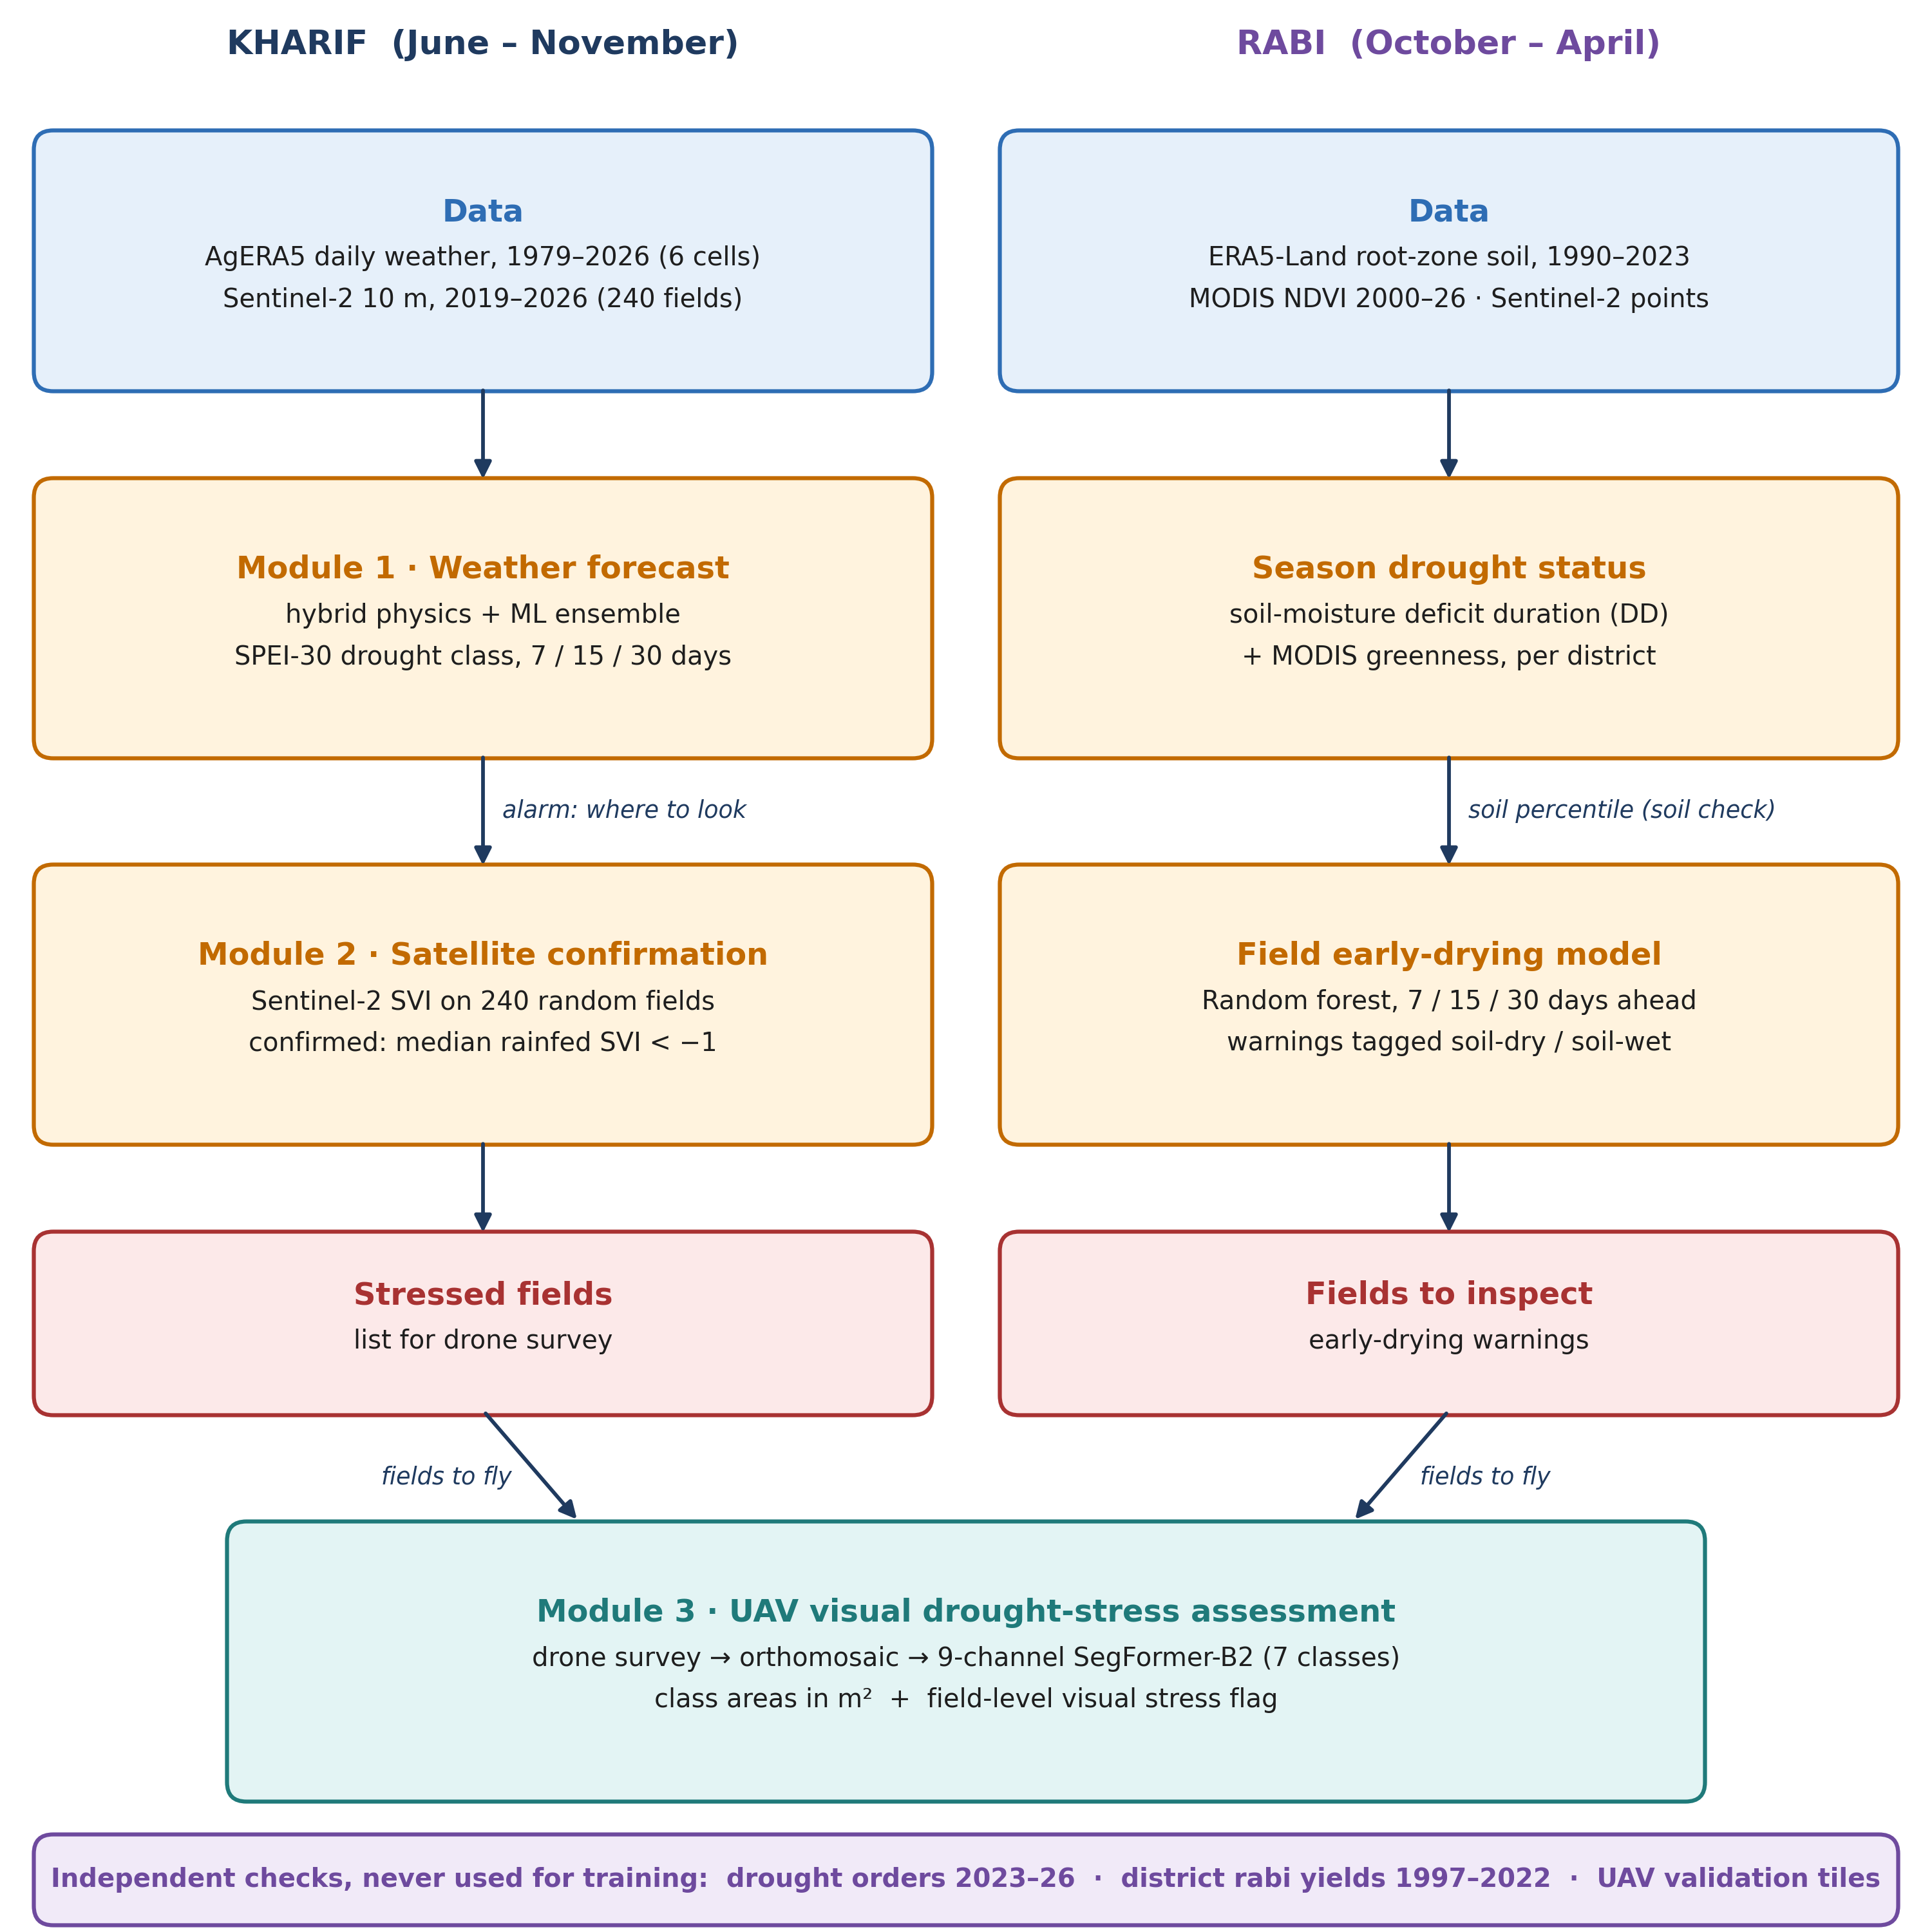
\includegraphics[width=0.8\textwidth]{figures/v2_system.png}
\caption{Overall architecture. Kharif: the weather forecast (Module 1) triggers the satellite check (Module 2), which lists stressed fields. Rabi: the season drought status and the field early-drying model list fields to inspect. Both lists go to the UAV module (Module 3).}
\label{fig:system}
\end{figure}

% ============================================================================
\section{Kharif Module: Weather Forecast and Satellite Confirmation}

\subsection{Weather forecasting (Module 1)}
\textbf{Labels.} The daily water balance $D_t = P_t - \mathrm{ET}_{0,t}$ is summed over 30 days and standardised to SPEI-30~\cite{vicente2010} with a log-logistic distribution fitted per site and month on \textbf{1979--2011 only} and then frozen. Classes: Healthy ($\ge 0$), Moderate ($-1.5$ to $0$), Severe ($< -1.5$); the target is the class on day $t+h$, $h \in \{7, 15, 30\}$.

\textbf{Hybrid model.} Inputs are a 30-day window of 9 weather variables, SPEI history and day of year, plus the class probabilities of a physical \textbf{water-balance ensemble}: the unknown days of the future SPEI window are filled with each 1979--2011 year's water balance,
\begin{equation}
\hat{p}_c = \frac{1}{|Y|}\sum_{y \in Y} \mathbf{1}\big[\text{class}(\mathrm{SPEI}^{(y)}_{t+h}) = c\big], \qquad Y = \{1979,\dots,2011\}.
\end{equation}
Random Forest~\cite{breiman2001}, XGBoost~\cite{chen2016}, LSTM and Transformer (5 seeds each) are combined by soft voting weighted on validation \mf. Split: train 1979--2011, validation 2012--2018, test 2019--2026, purged so no sample crosses a boundary (Fig.~\ref{fig:w_arch}).

\begin{figure}[!htbp]
\centering
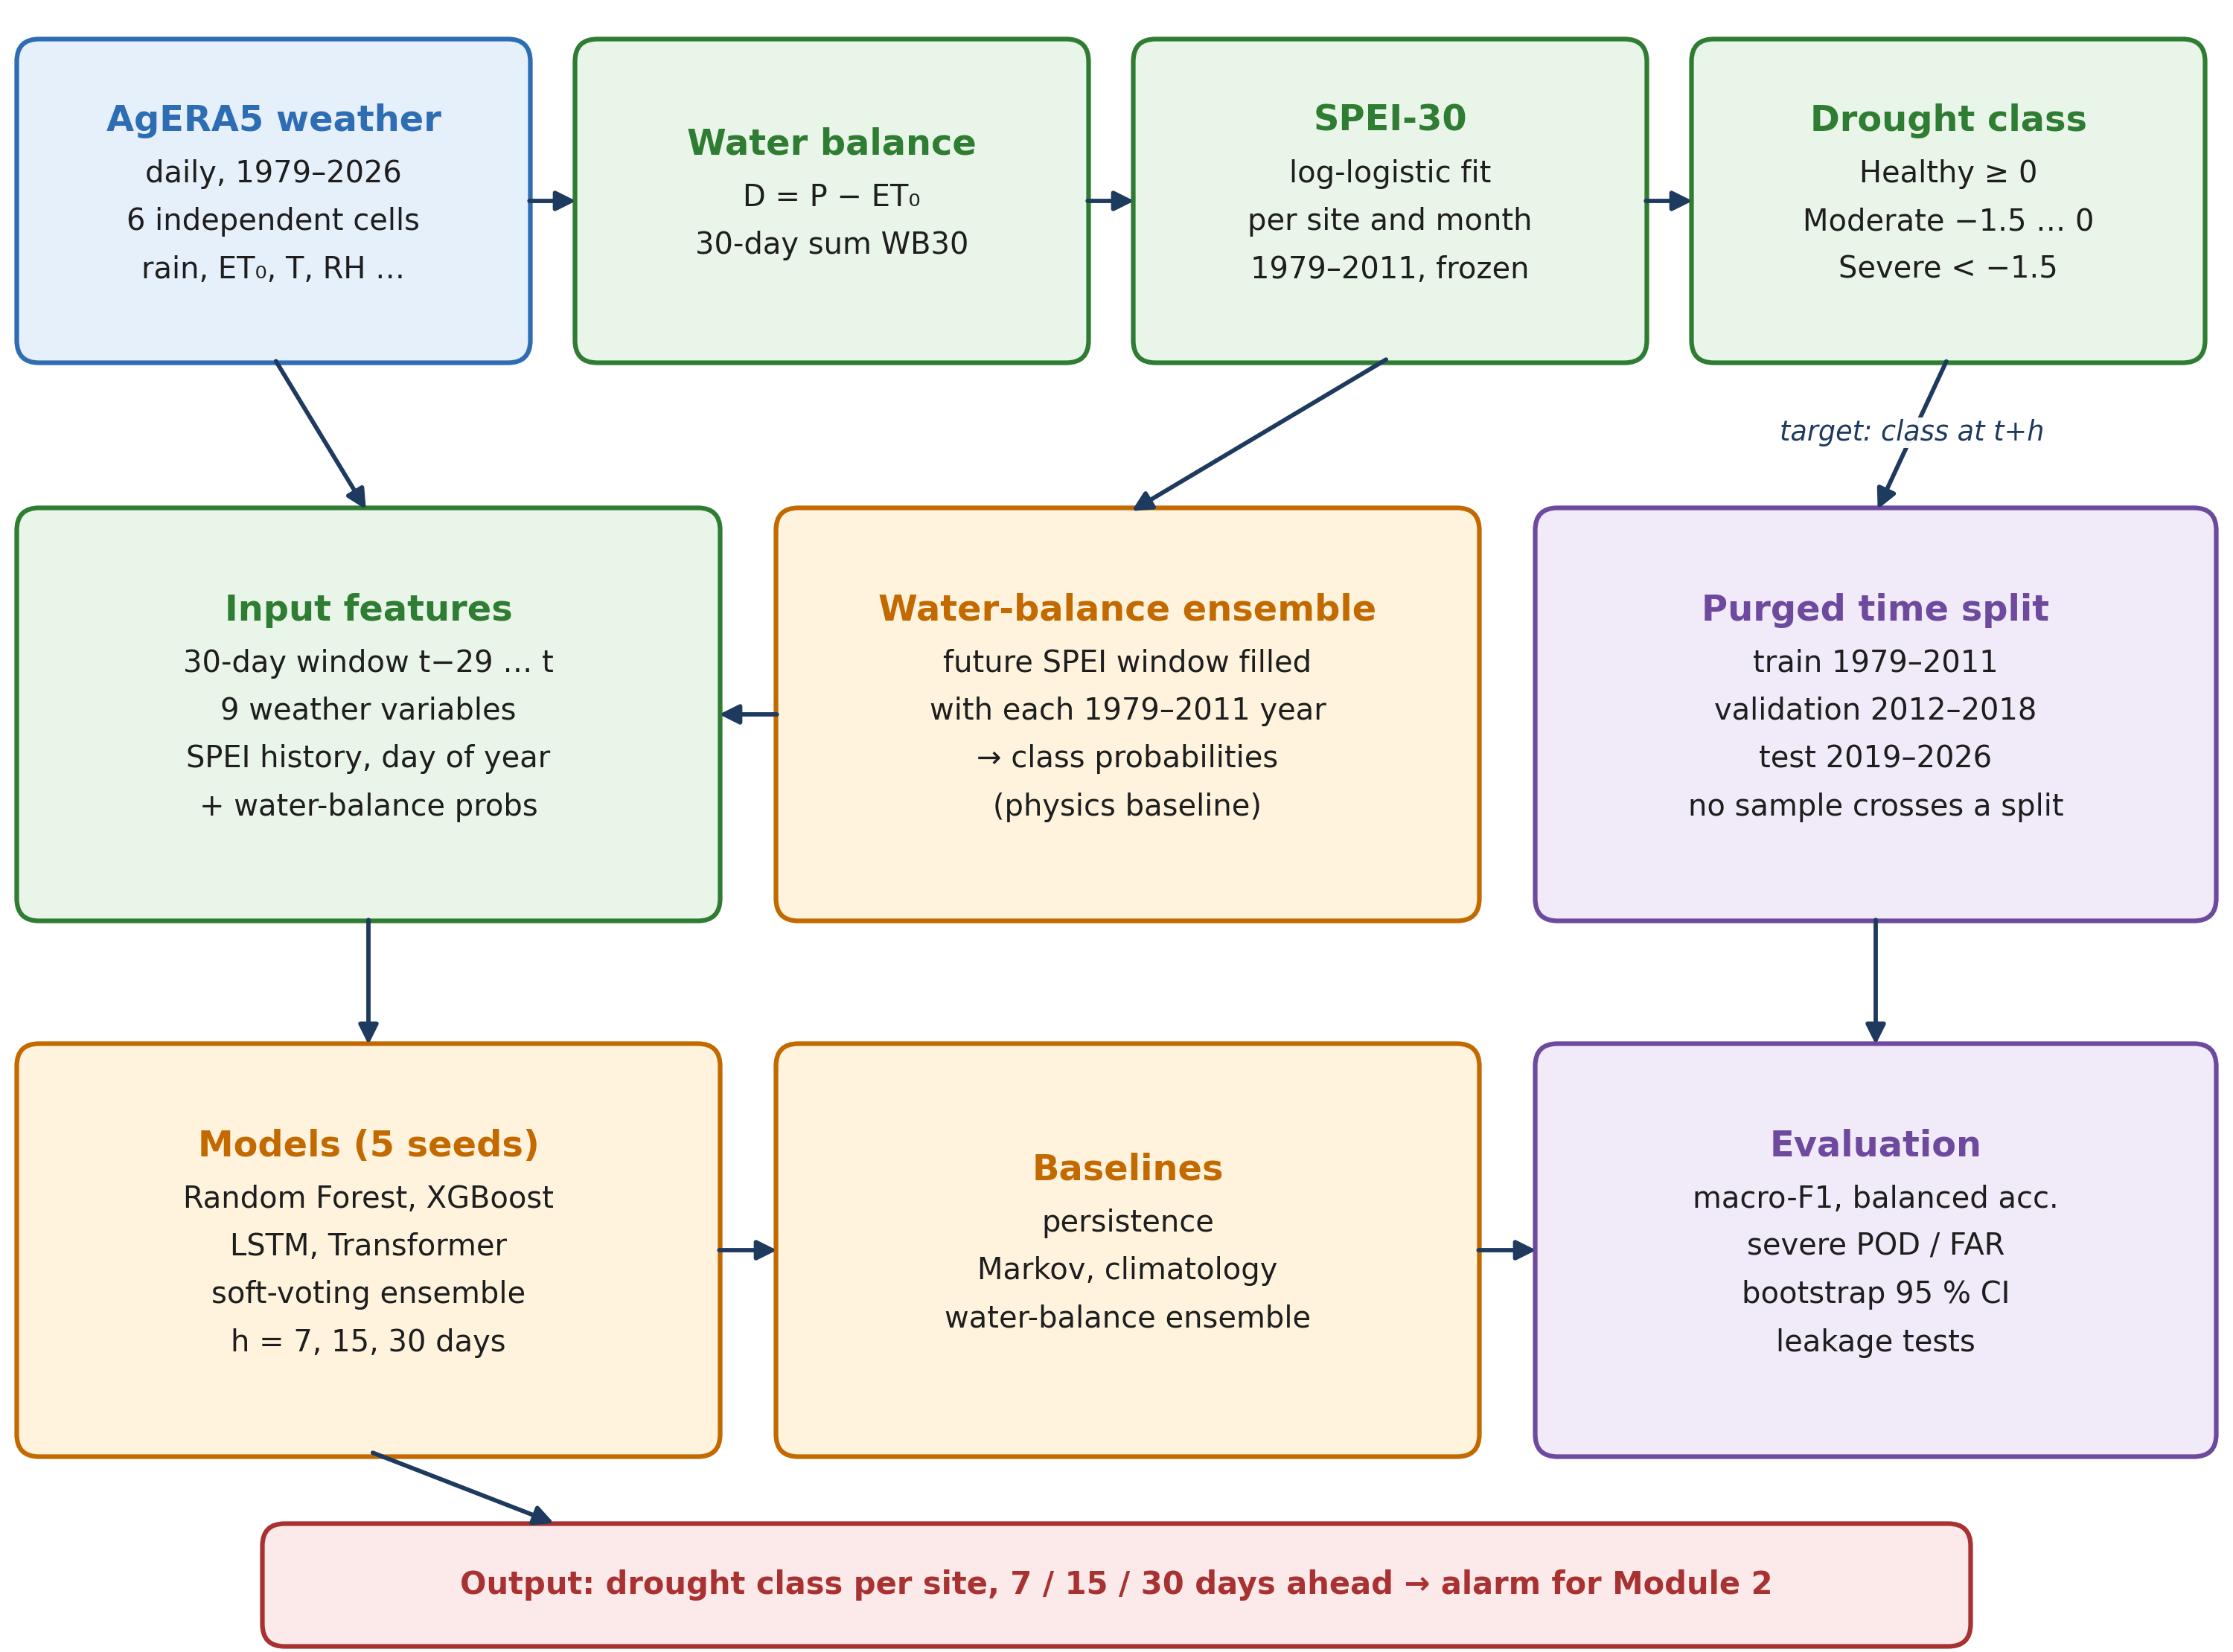
\includegraphics[width=0.92\textwidth]{figures/v2_weather.png}
\caption{Weather module architecture.}
\label{fig:w_arch}
\end{figure}

\begin{table}[!htbp]
\centering
\caption{Weather module, test 2019--2026, all sites (\mf; models mean of 5 seeds).}
\label{tab:w}
\footnotesize
\begin{tabular}{|l|c|c|c|}
\hline
\textbf{Model} & \textbf{7 days} & \textbf{15 days} & \textbf{30 days} \\
\hline
Persistence (class today) & 0.662 & 0.515 & 0.424 \\ \hline
Water-balance ensemble (physics only) & 0.783 & 0.592 & 0.375 \\ \hline
Best model without physics input (XGBoost) & 0.755 & 0.613 & 0.424 \\ \hline
XGBoost / LSTM / Transformer, hybrid & 0.814 / 0.806 / 0.809 & 0.631 / 0.642 / 0.650 & 0.418 / 0.406 / 0.407 \\ \hline
\textbf{Soft-voting ensemble, hybrid} & \textbf{0.819} & \textbf{0.651} & \textbf{0.424} \\ \hline
Balanced accuracy / ROC-AUC, hybrid & 85.6\,\% / 0.97 & 68.3\,\% / 0.90 & 42.5\,\% / 0.68 \\
\hline
\end{tabular}
\end{table}

The hybrid beats persistence at 7 and 15 days and the physics model significantly at 15 days (95\,\% CI of the gain [+0.010, +0.099]). The water-balance probabilities are the most valuable single input (+0.063 at 7 days). For severe drought, 80\,\% of severe days are detected 7 days ahead (false-alarm ratio 0.34). At 30 days no model beats persistence, and this is reported as a limit.

\begin{figure}[!htbp]
\centering
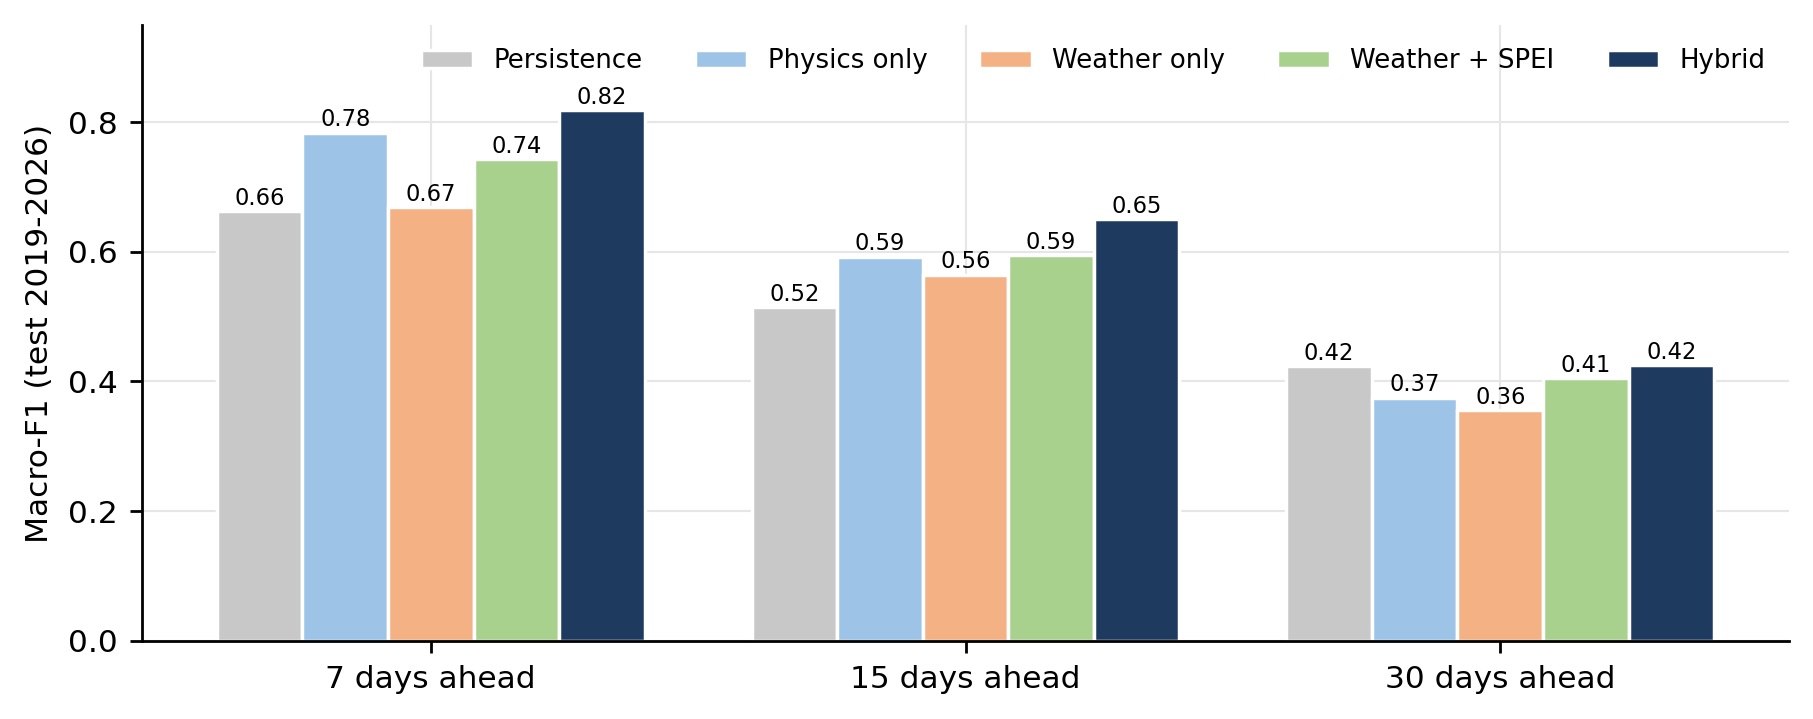
\includegraphics[width=0.78\textwidth]{figures/res_w_bars.png}
\caption{Weather module \mf{} on the test years 2019--2026: persistence, the physical water-balance ensemble and the ensemble model with three input sets. Physics inputs give the largest gain.}
\label{fig:w_bars}
\end{figure}

\subsection{Satellite confirmation (Module 2)}
Farmland within 3\,km of each site is mapped in Earth Engine (WorldCover cropland minus built-up, trees and water) and split into field segments~\cite{achanta2017}; a seeded random sample gives \textbf{240 fields} (20 rainfed, 10 irrigated per site). Crop condition is the Standardized Vegetation Index~\cite{peters2002}
\begin{equation}
\mathrm{SVI}_{f,d} = \big(\mathrm{NDVI}_{f,d} - \mu_{f,\mathrm{doy}(d)}\big) / \sigma_{f,\mathrm{doy}(d)},
\end{equation}
with normals from images up to 2023 and the scored year removed (Fig.~\ref{fig:s_arch}). Rainfed SVI follows SPEI-30 with a \textbf{10-day lag} ($\rho = 0.48$ on 2019--2023, 0.45 on unseen 2024--2026). A 15-day crop-condition forecast (XGBoost on satellite history plus the weather module's forecast) reaches \mf{} 0.67 vs 0.65 for persistence, and ranks fields that will become stressed at onset ROC-AUC 0.76 (logistic baseline 0.72; Random Forest on the same inputs 0.67 and 0.73).

\begin{figure}[!htbp]
\centering
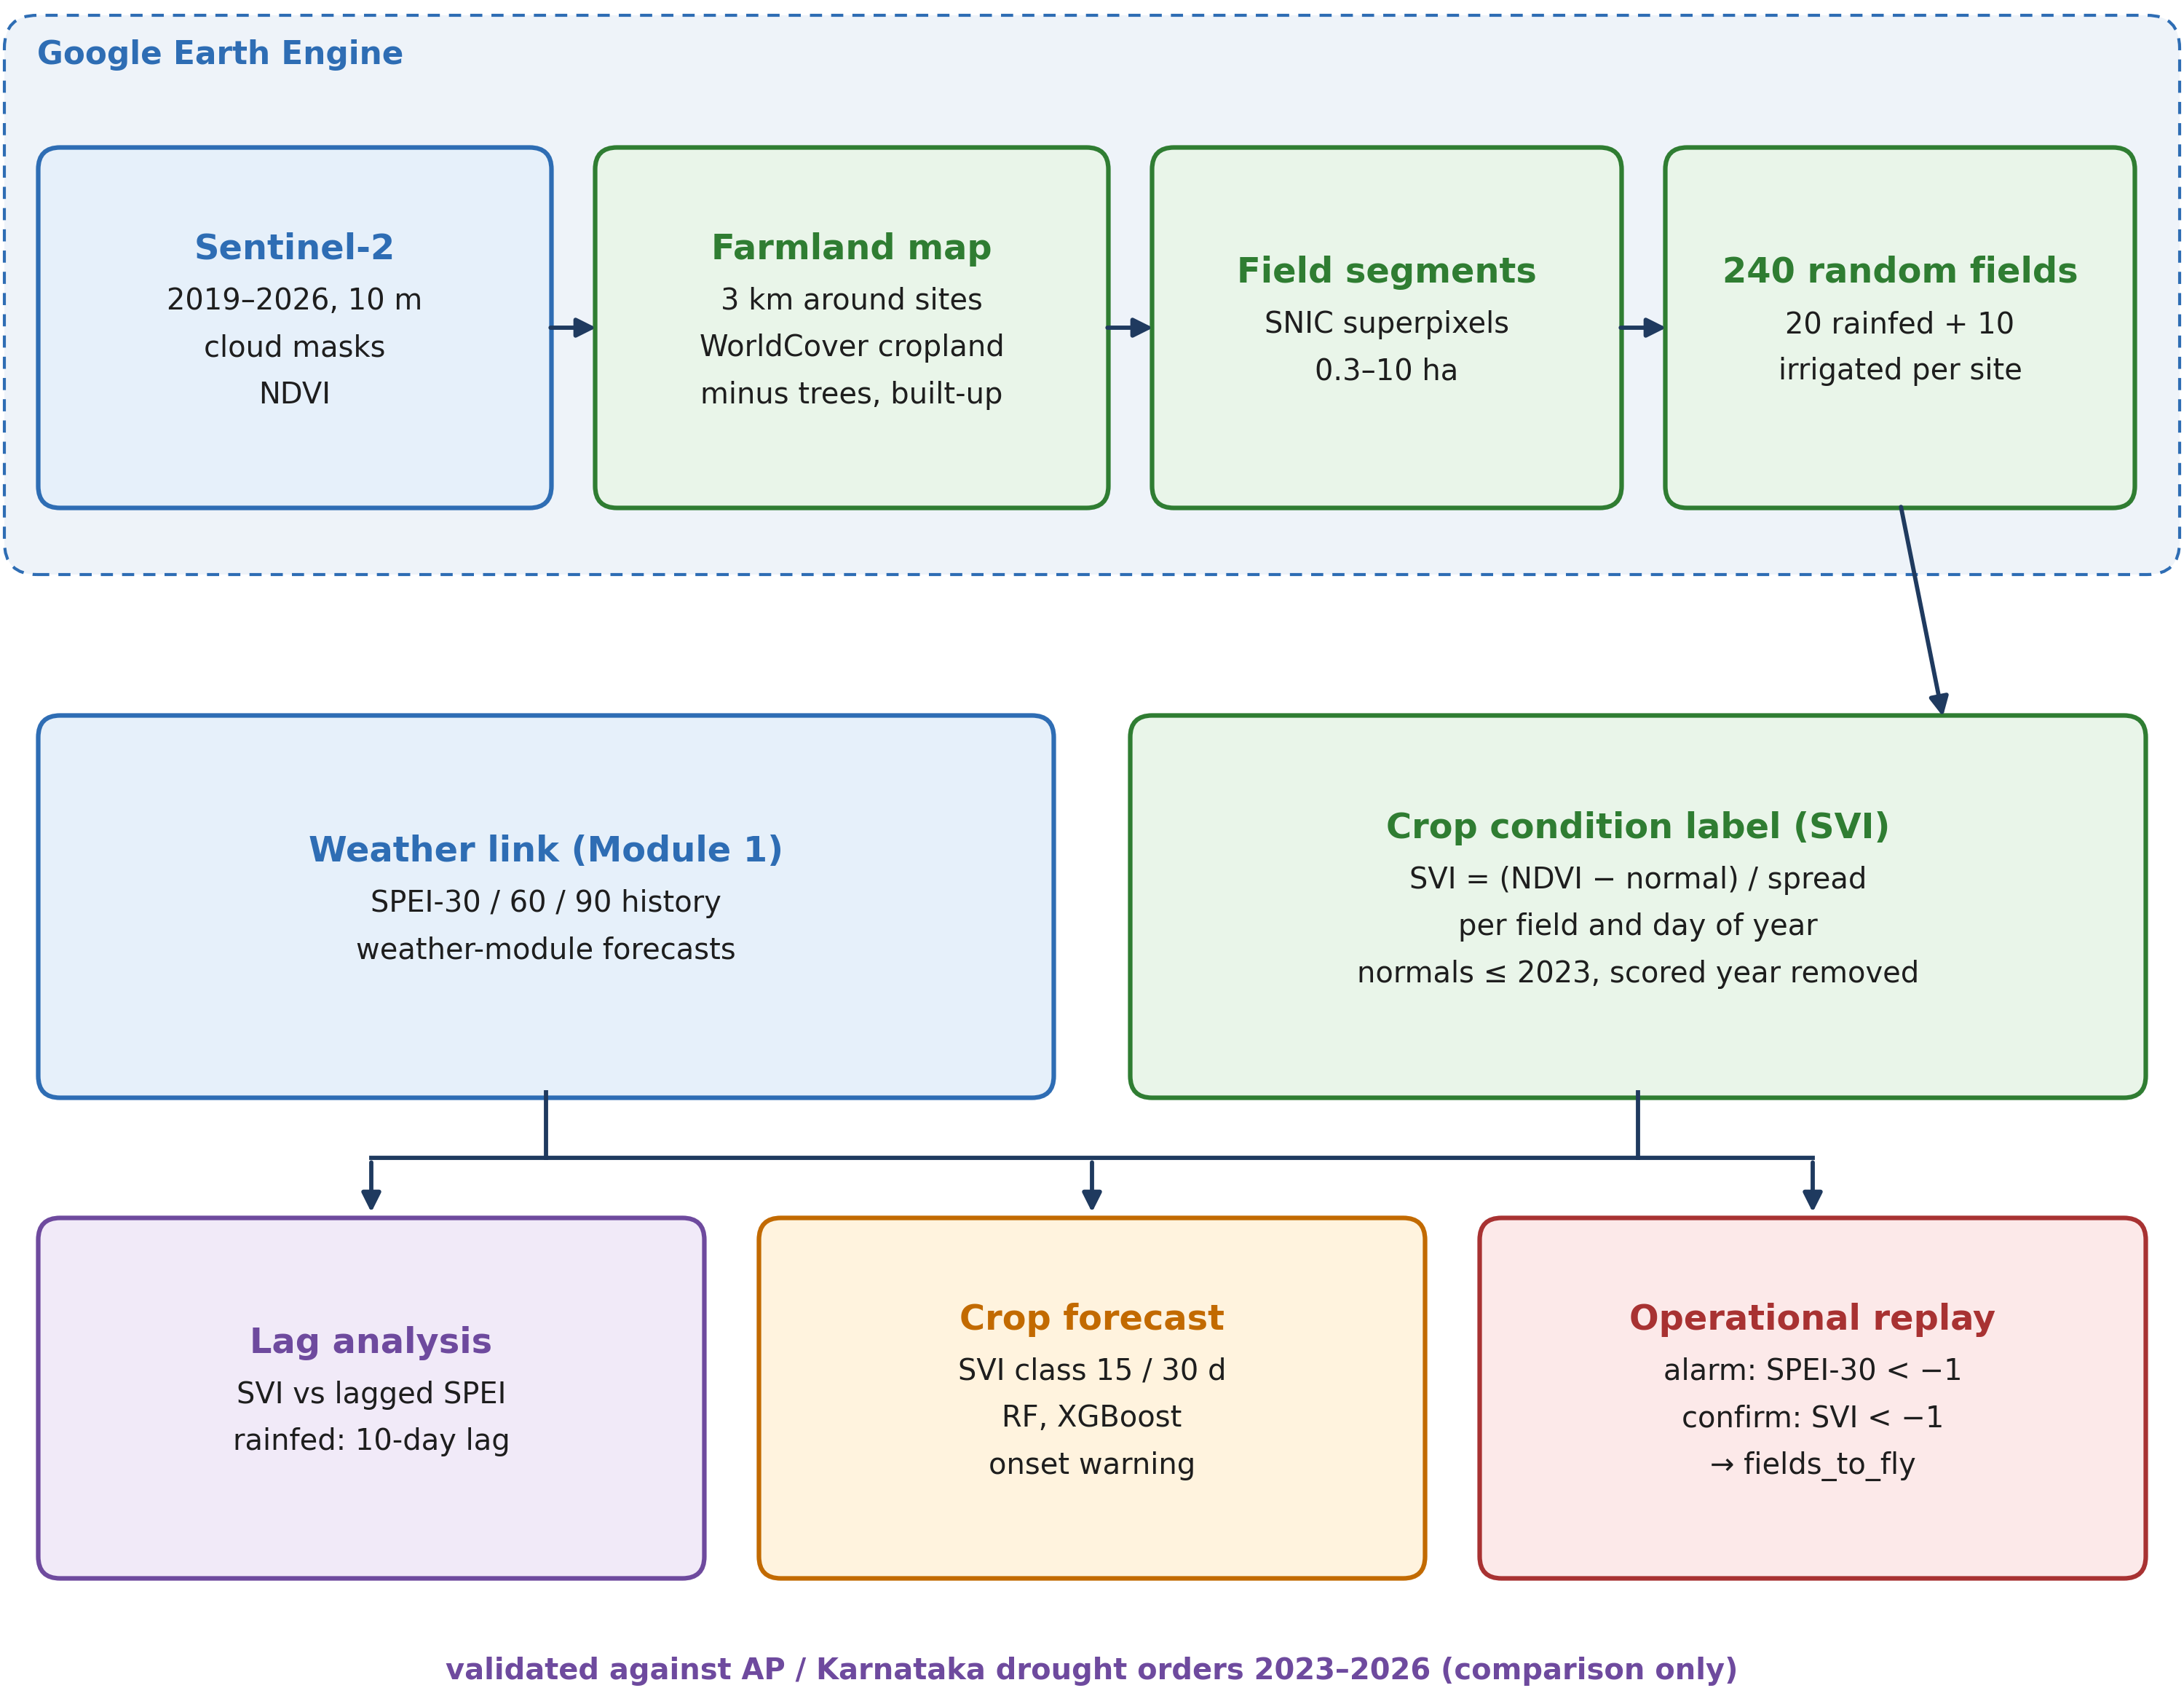
\includegraphics[width=0.85\textwidth]{figures/v2_satellite.png}
\caption{Satellite module architecture; its output \texttt{fields\_to\_fly} is the hand-off to the UAV module.}
\label{fig:s_arch}
\end{figure}

\subsection{Combined kharif chain: replay against government orders}
The chain was replayed every 5 days from June to November without retraining, using weather 7 days late and satellite 2 days late. \emph{Alarm} = SPEI-30 $< -1$ or a severe 15-day forecast; \emph{confirmed} = median rainfed SVI $< -1$ over at least 5 clear fields.

\begin{table}[H]
\centering
\caption{Operational replay vs official kharif declarations, 2023--2026 (2023 retrospective, 2024--2026 prospective).}
\label{tab:replay}
\footnotesize
\begin{tabular}{|l|c|c|c|c|}
\hline
\multirow{2}{*}{\textbf{Official decision}} & \multicolumn{2}{c|}{\textbf{Site-seasons}} & \multicolumn{2}{c|}{\textbf{Mandal-seasons}} \\
\cline{2-3}\cline{4-5}
 & \textbf{confirmed} & \textbf{before order} & \textbf{confirmed} & \textbf{before order} \\
\hline
Severe & 9 / 9 & 5 / 9 & 6 / 6 & 5 / 6 \\ \hline
Moderate & 3 / 6 & 3 / 6 & 2 / 4 & 2 / 4 \\ \hline
Not declared (false alarm) & 1 / 11 & & 1 / 8 & \\
\hline
\end{tabular}
\end{table}
All severe droughts were confirmed, two of them 22 days before the order (2026). The 2025 moderate declarations were missed: rain was above normal and crops stayed green during the replay window. Applied unchanged to rabi, the chain confirmed none of the 4 severe rabi mandal-seasons, which motivated the separate rabi module.

Figure~\ref{fig:s_cases} shows four replayed seasons. At Balaji Villas (2023) and Dinnedevarapadu (2026) the weather alarm came first, crop SVI then fell below $-1$ and drought was confirmed before the order; at Somandepalle (2025, declared moderate) rain was above normal and crops stayed green, so the system stayed silent.

\begin{figure}[!htbp]
\centering
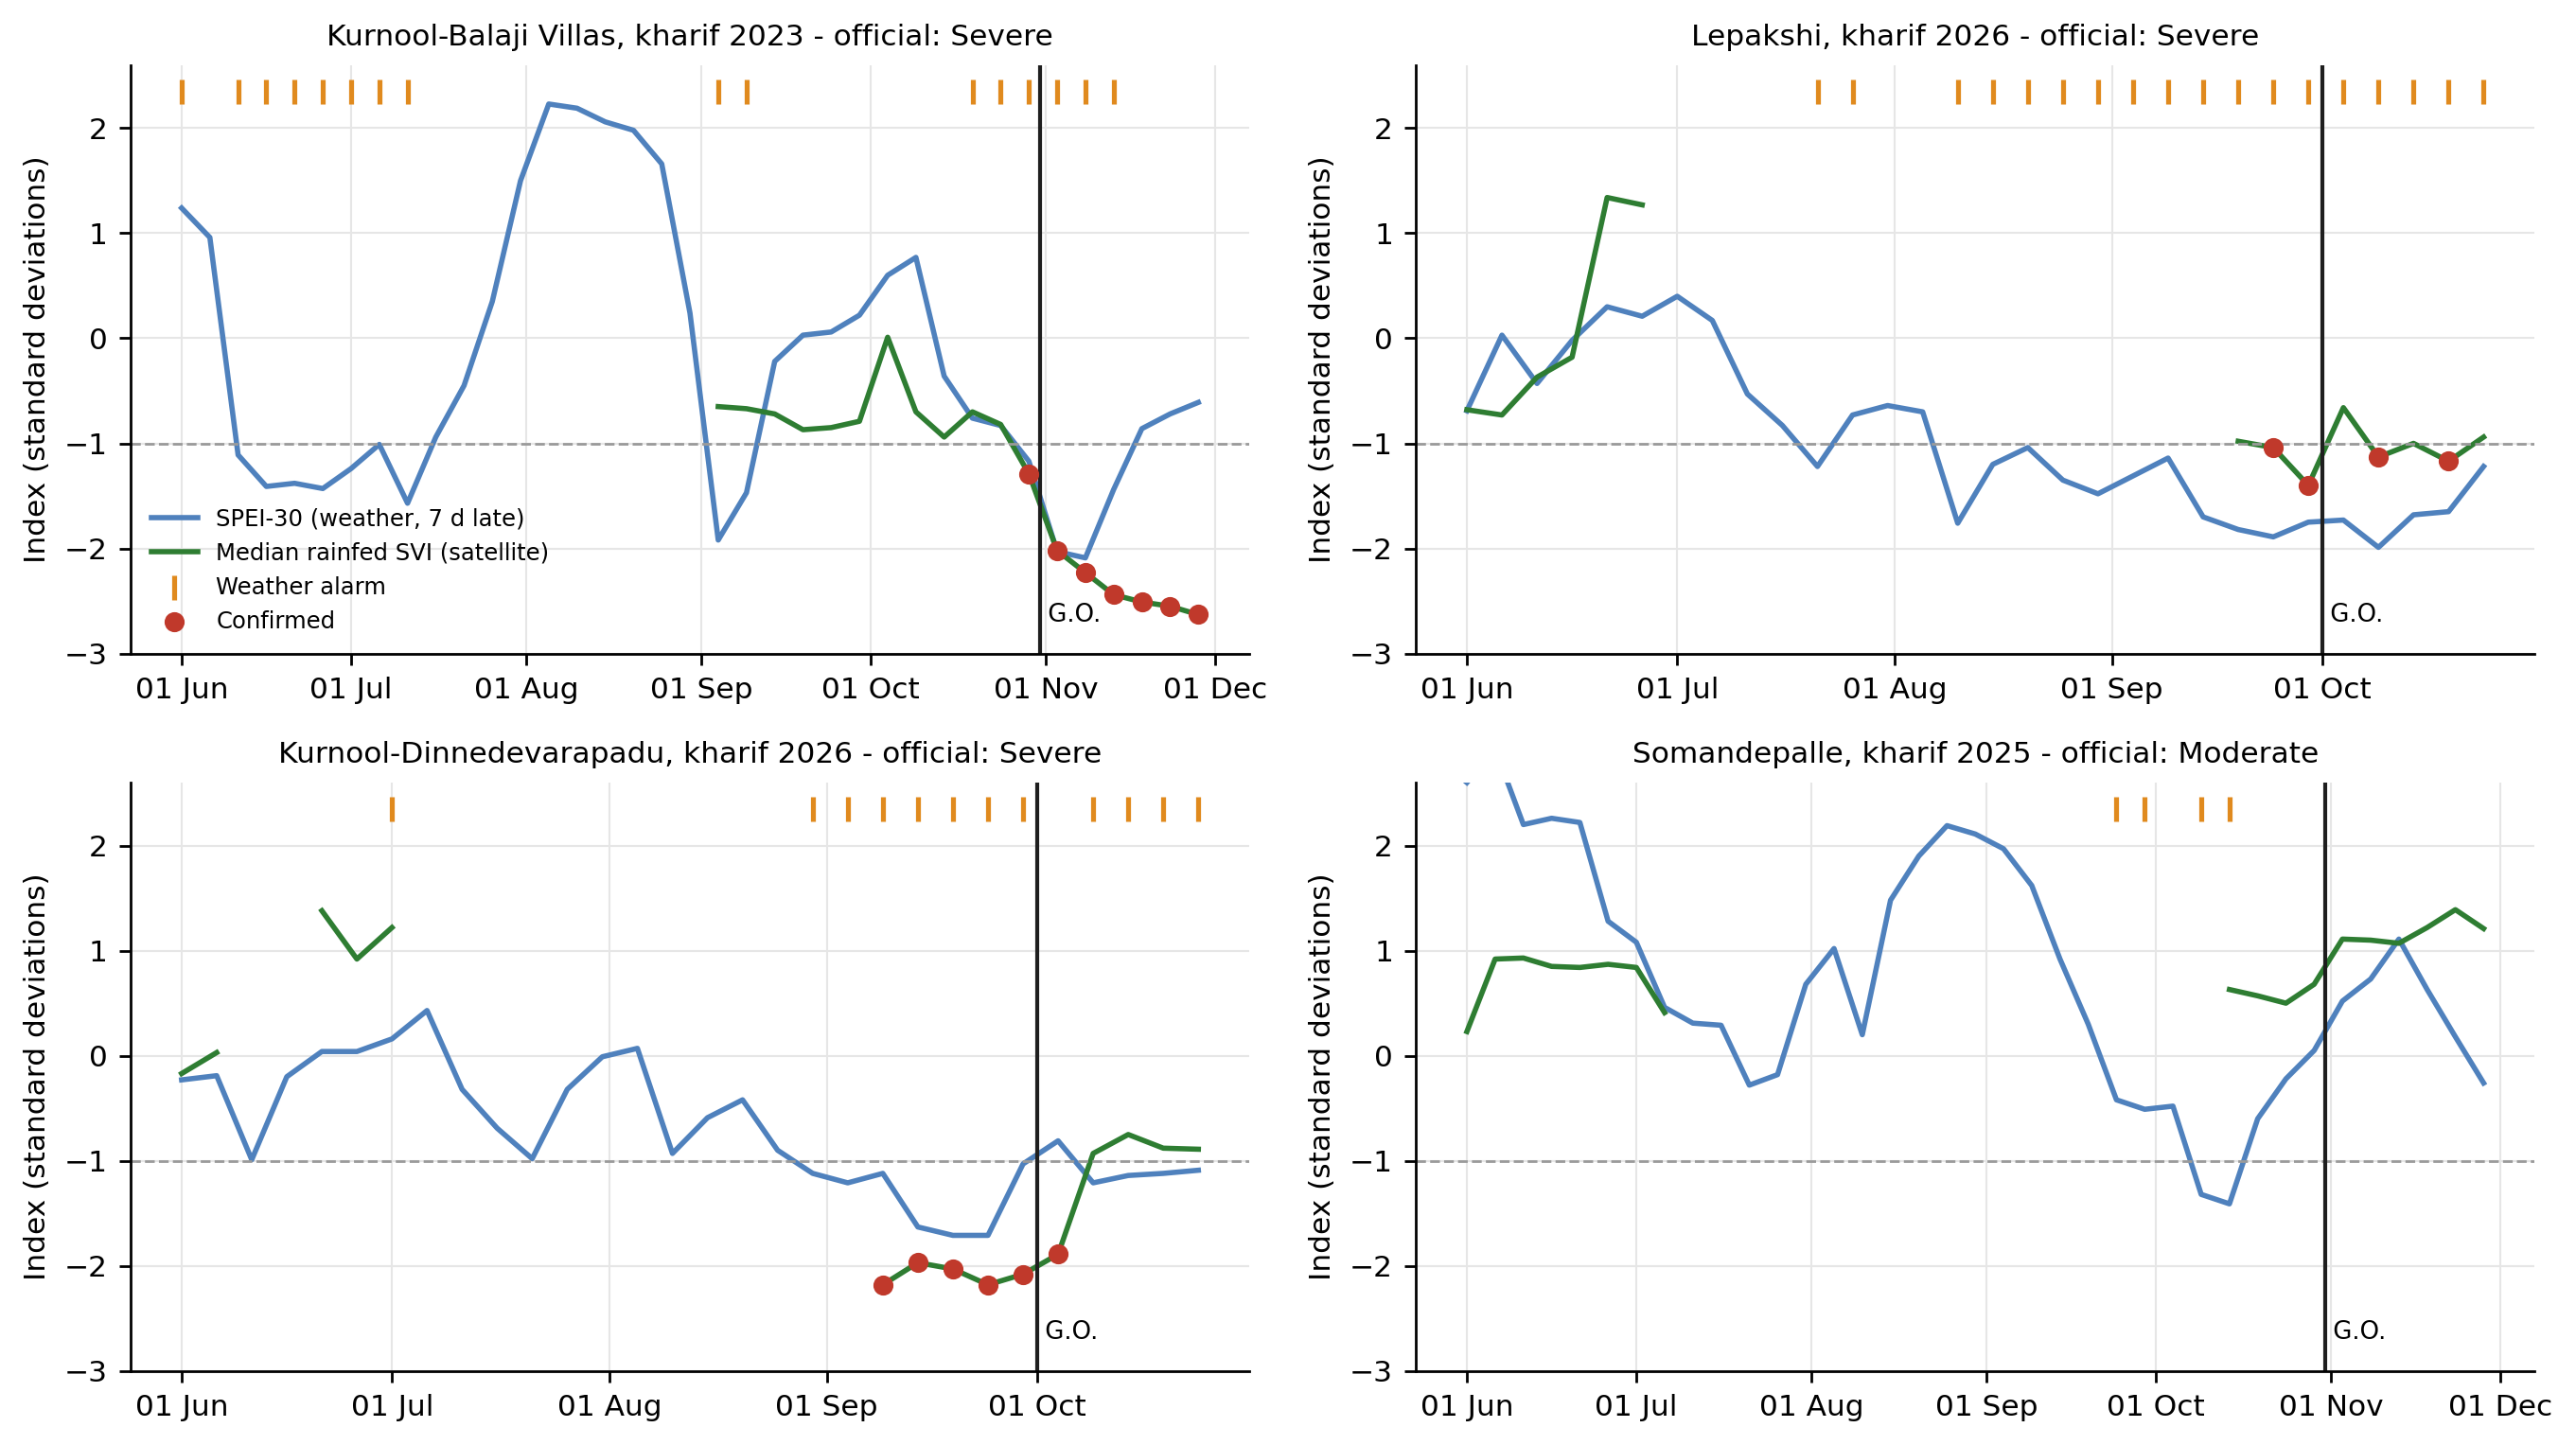
\includegraphics[width=0.7\textwidth]{figures/res_s_cases.png}
\caption{Replay case studies: SPEI-30 available on each issue date (blue), median rainfed SVI (green), weather alarms (orange ticks), confirmed drought (red dots) and the government order date (G.O., black line).}
\label{fig:s_cases}
\end{figure}

% ============================================================================
\section{Rabi Module}
\textbf{Why a separate rabi module.} The kharif chain (weather $\rightarrow$ satellite) does not work in rabi, for four reasons:
\begin{enumerate}
\item \textbf{Different water source.} Rabi crops (October--April) grow mainly on water stored in the soil after the monsoon, plus irrigation and little rain, and soil moisture is the largest contributor to agricultural drought in the region~\cite{kulkarni2020}. A rain-based index such as SPEI does not measure this: in-season rain (November--February) is unrelated to rabi yields ($\rho = +0.01$, Table~\ref{tab:r_dd}).
\item \textbf{The kharif chain failed in rabi.} Applied unchanged to rabi 2023--2026, it confirmed \textbf{none} of the 4 severe rabi mandal-seasons declared by the government.
\item \textbf{Too few rabi declarations to learn from.} Only 4 severe rabi mandal-seasons exist in our area, far too few to train or test a model on government orders.
\item \textbf{Harvest looks like drought.} In rabi, greenness falls at harvest (January--March) as well as in drought, so a greenness drop alone cannot be trusted.
\end{enumerate}
The rabi module therefore measures \textbf{root-zone soil moisture}, uses it to tell drought from harvest, and is validated against an independent outcome, \textbf{district crop yields} over 1997--2022, instead of a few declarations (Fig.~\ref{fig:r_arch}).

\begin{figure}[!htbp]
\centering
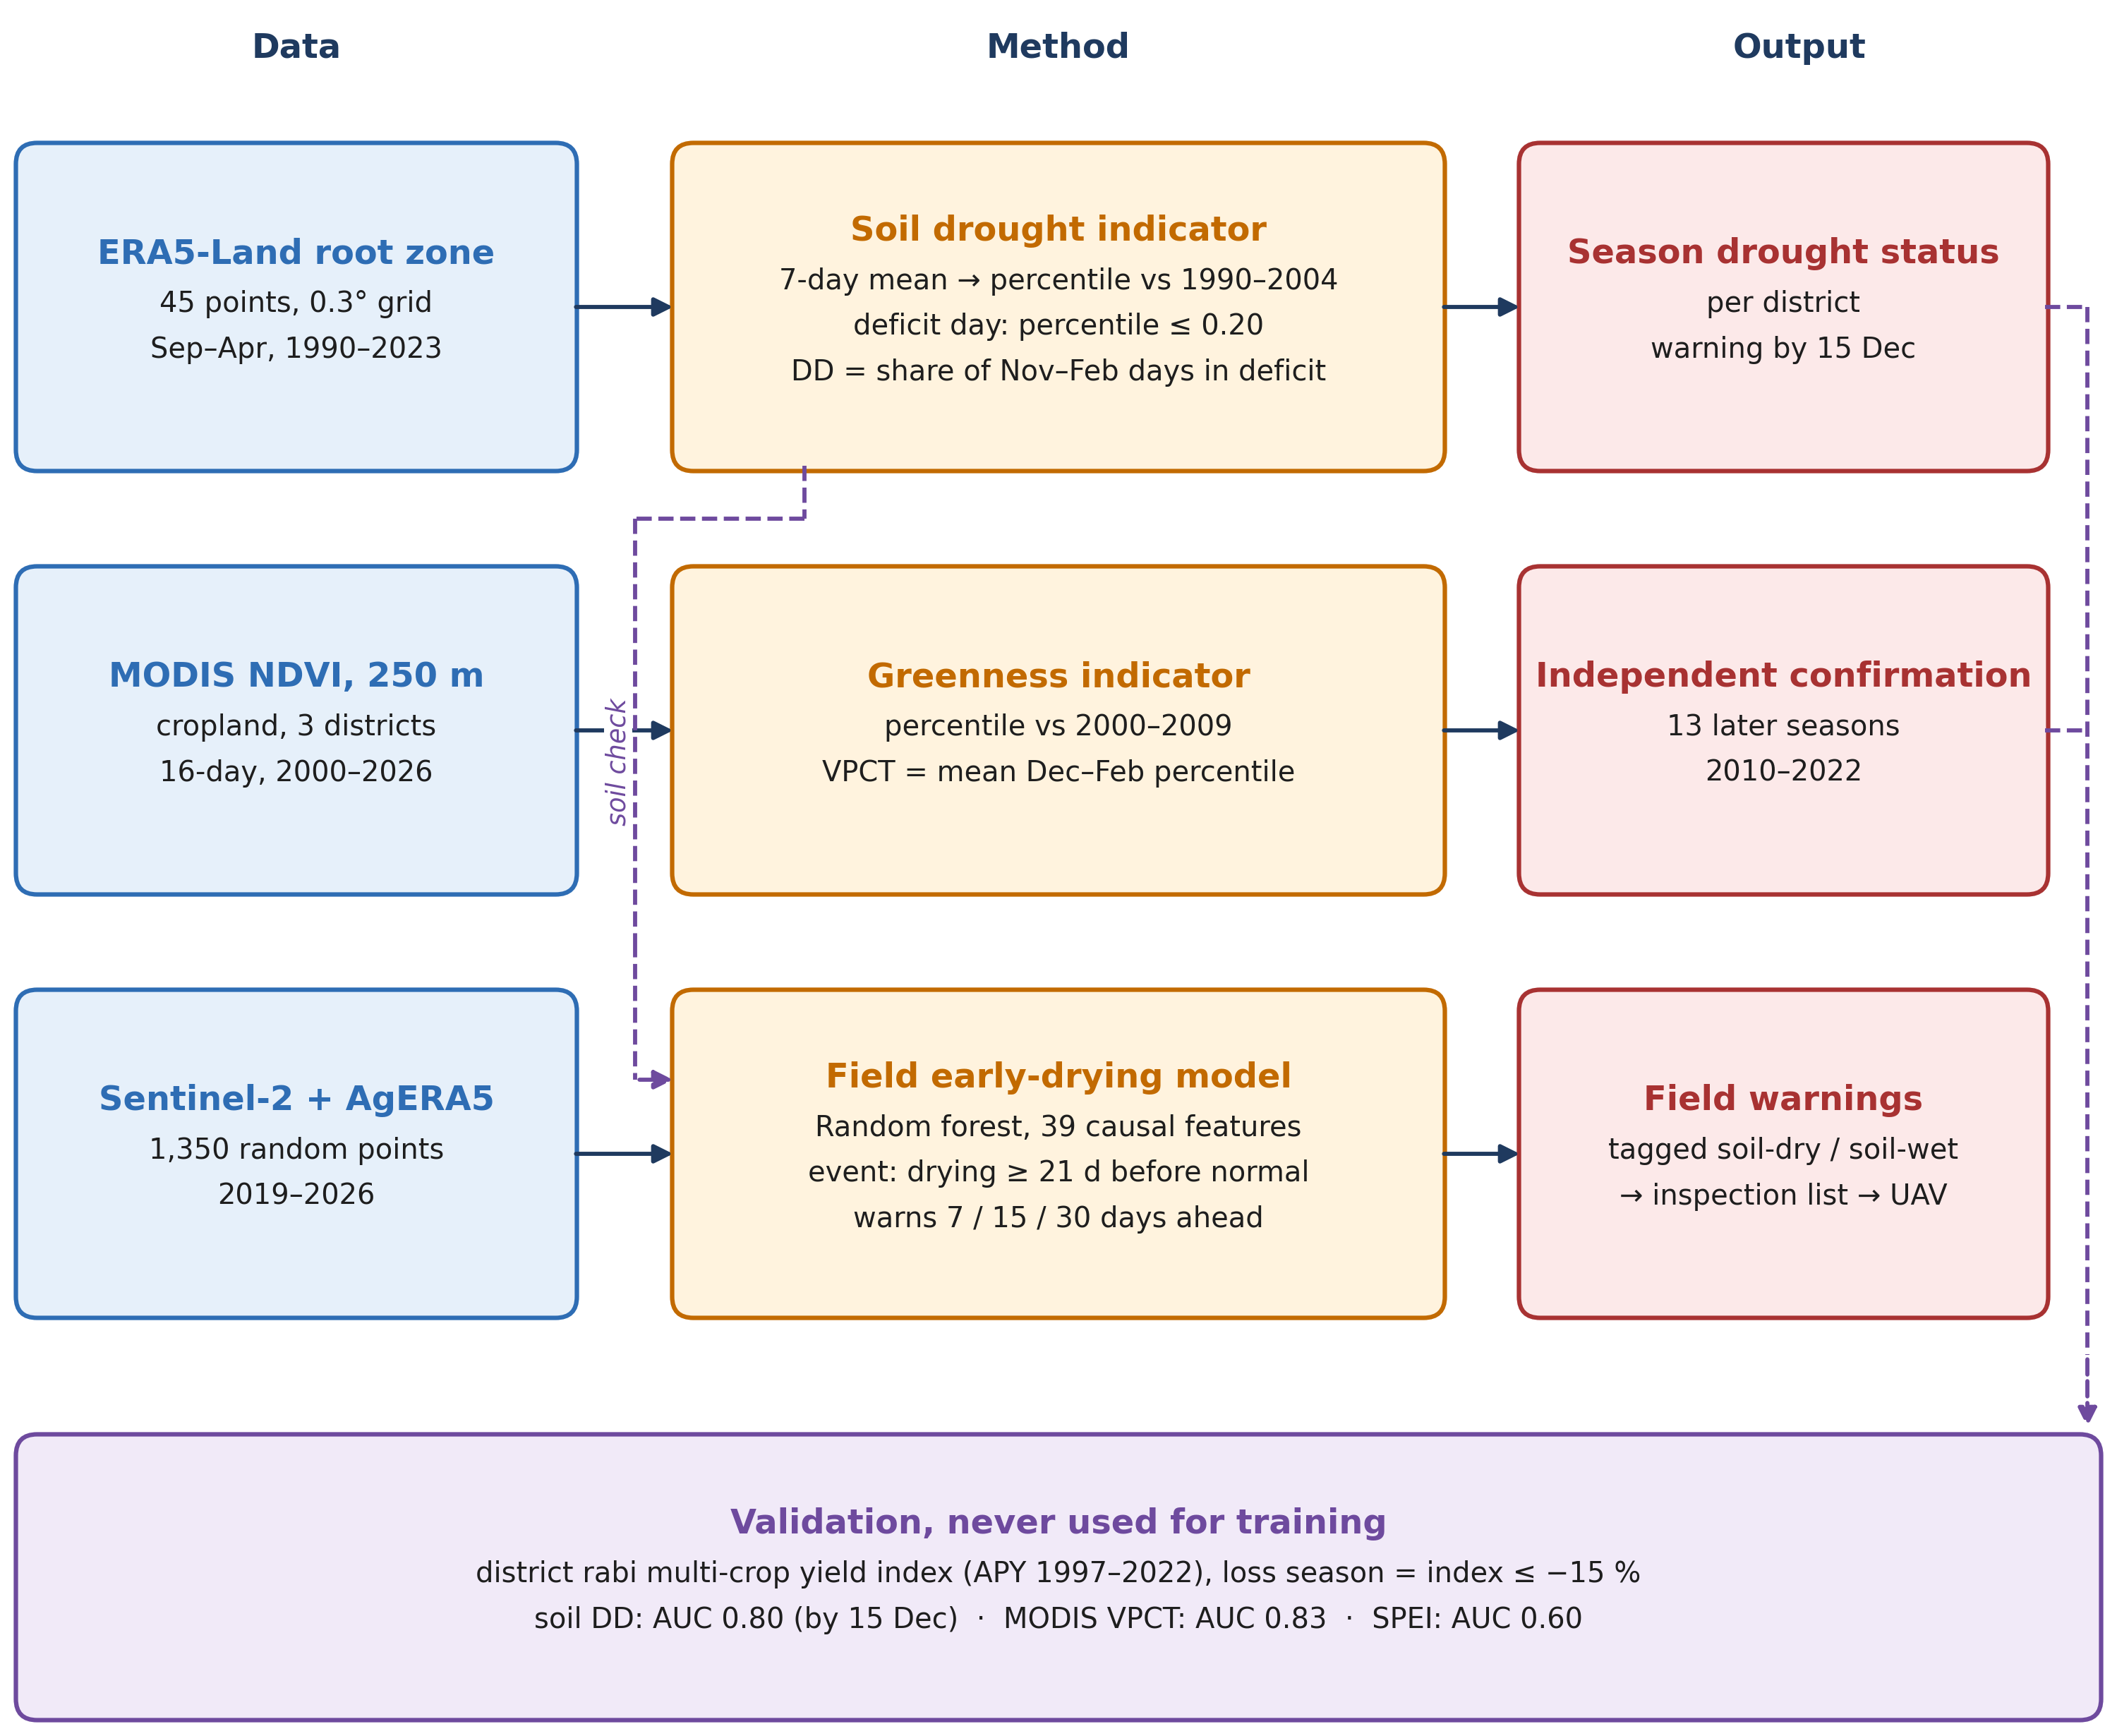
\includegraphics[width=0.8\textwidth]{figures/v2_rabi.png}
\caption{Rabi module. The soil percentile also tags each field warning as soil-dry or soil-wet (dashed). Season-level outputs are validated against district crop yields.}
\label{fig:r_arch}
\end{figure}

\textbf{Soil drought indicator.} Root-zone moisture $\theta = 0.07\,\theta_{0-7} + 0.21\,\theta_{7-28} + 0.72\,\theta_{28-100}$ (cm) is averaged over 7 days and turned into a percentile against the same point and calendar window ($\pm 15$ days) in 1990--2004. A day is in deficit if the percentile is $\le 0.20$. \textbf{Deficit duration} DD is the share of 1 November -- 28 February days in deficit, averaged over the district's points. \textbf{Outcome:} a multi-crop rabi \emph{yield index} (each major crop's yield relative to the median of its previous 5 seasons, fixed area weights); a \emph{loss season} has index $\le -15\,\%$. Early-warning inputs end 8 days before the issue date.

\begin{table}[!htbp]
\centering
\caption{Rabi indicators vs independent district crop outcomes, Kurnool + Anantapur (within-district Spearman $\rho$; AUC for the 11 loss seasons among 46 district-seasons; 95\,\% CI resampling whole seasons).}
\label{tab:r_dd}
\footnotesize
\begin{tabular}{|l|c|c|}
\hline
\textbf{Indicator} & \textbf{$\rho$ with yield index, 2000--2022} & \textbf{Loss-season AUC, issued 15 Dec} \\
\hline
\textbf{Soil deficit duration (DD)} & $\mathbf{-0.58}$ [$-0.74$, $-0.36$] & \textbf{0.80} [0.62, 0.95] \\ \hline
Soil moisture at sowing (Oct--Nov) & $+0.55$ [$+0.27$, $+0.73$] & 0.77 [0.58, 0.93] \\ \hline
Rain June--November & $+0.40$ [$+0.07$, $+0.63$] & 0.72 [0.51, 0.89] \\ \hline
SPEI-30 (Oct--Nov; so far at issue) & $+0.44$ [$+0.10$, $+0.68$] & 0.60 [0.36, 0.80] \\ \hline
Rain November--February (in season) & $+0.01$ [$-0.35$, $+0.39$] & -- \\
\hline
\end{tabular}
\end{table}

\textbf{Independent greenness check.} With rules written before the MODIS data was downloaded, we compared the mean Dec--Feb NDVI percentile (VPCT, vs 2000--2009) on the 13 later seasons 2010--2022: VPCT relates to yield at $\rho = +0.70$ [0.25, 0.92] and detects loss seasons at \textbf{AUC 0.83} (0.81 already by 15 January), as well as soil DD on the same seasons (0.82) and better than SPEI (0.65). Two loss seasons with wet soil and green crops (Anantapur 2015, 2021) are flagged by neither, consistent with losses not caused by drought. A planned test of ``low greenness + dry soil'' could not be run: the districts became greener after 2010 (Dec--Feb NDVI 0.32 $\rightarrow$ 0.40 in Anantapur), so few seasons fell below the fixed 2000--2009 reference.

\begin{figure}[!htbp]
\centering
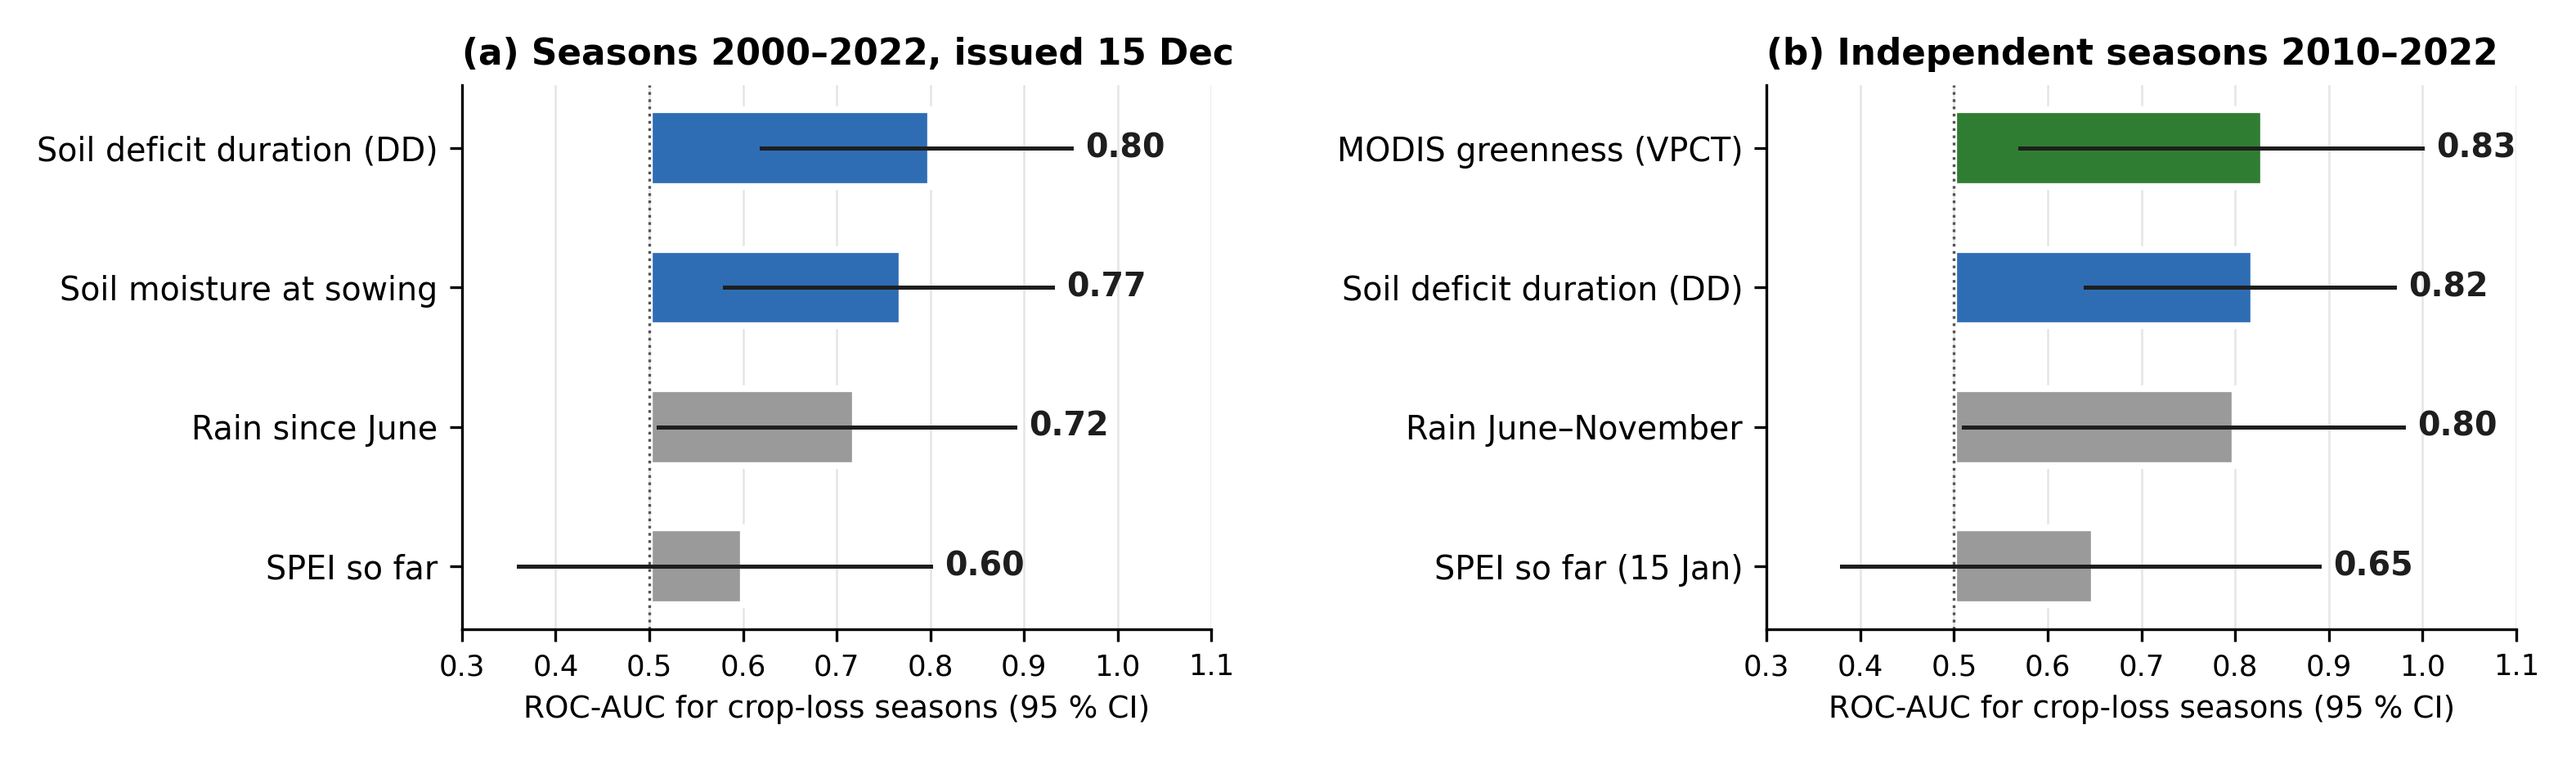
\includegraphics[width=0.88\textwidth]{figures/rabi_auc.png}
\caption{How well each rabi indicator separates crop-loss seasons from normal seasons (ROC-AUC with 95\,\% CI; dotted line = no skill). Soil and greenness indicators (blue, green) beat the rain-based indices (grey), most clearly SPEI.}
\label{fig:r_auc}
\end{figure}

\textbf{Field early-drying model.} On 1,350 random Sentinel-2 cropland points, an event is an established crop drying $\ge$ 21 days before the point's normal drying date. A Random forest on 39 causal features (NDVI history, phenology, weather, root-zone soil) warns 7/15/30 days ahead; model and thresholds are chosen on validation season 2022 only (train 2019--2021, test 2023--2025, 108 events). Each warning is tagged \emph{soil-dry} if the soil percentile is below the cell's normal.

\begin{table}[H]
\centering
\caption{Field early-drying warnings, 30 days ahead, test 2023--2025 (108 events). Precision = share of warned point-seasons with a timely event.}
\label{tab:r_ed}
\footnotesize
\renewcommand{\arraystretch}{1.25}
\begin{tabular}{|l|c|c|c|}
\hline
\textbf{Model / operating point} & \textbf{Precision} & \textbf{Recall} & \textbf{Median lead} \\ \hline
Final model, validation-selected threshold & 0.54 [0.42, 0.66] & 0.28 [0.20, 0.36] & 16 days \\ \hline
\multicolumn{4}{|c|}{\textit{Comparison at the same number of events caught (40 of 108); threshold varied}} \\ \hline
Earlier model (21 features, no soil) & 0.51 & 0.37 & -- \\ \hline
Final model (39 features) & 0.56 & 0.37 & -- \\ \hline
\textbf{Final model, soil-dry warnings only} & \textbf{0.69} & 0.37 & -- \\ \hline
\end{tabular}
\end{table}
Warnings issued under below-normal soil are correct about twice as often as under wet soil (0.67 vs 0.38), where greenness drops are mostly harvest. Because these test seasons had been examined during development and only 2023 had below-normal soil, this contrast is descriptive. A separate XGBoost forecast of NDVI 15 days ahead has 18\,\% lower error than the best simple baseline on three held-out seasons (MAE 0.051 vs 0.062).

% ============================================================================
\section{UAV Module: Visual Drought-Stress Segmentation}

The UAV module has two phases (Fig.~\ref{fig:u_pipe}). In phase A, drone photos are labelled semi-automatically and a segmentation model is trained (steps 1--8). In phase B, each field's orthomosaic is segmented tile by tile, stitched, cleaned, measured and reported (steps 9--15). Note the two kinds of stitching: Metashape stitches \emph{photos} into an orthomosaic (step 9), while our pipeline stitches \emph{predictions} of overlapping tiles (step 11).

\begin{figure}[!htbp]
\centering
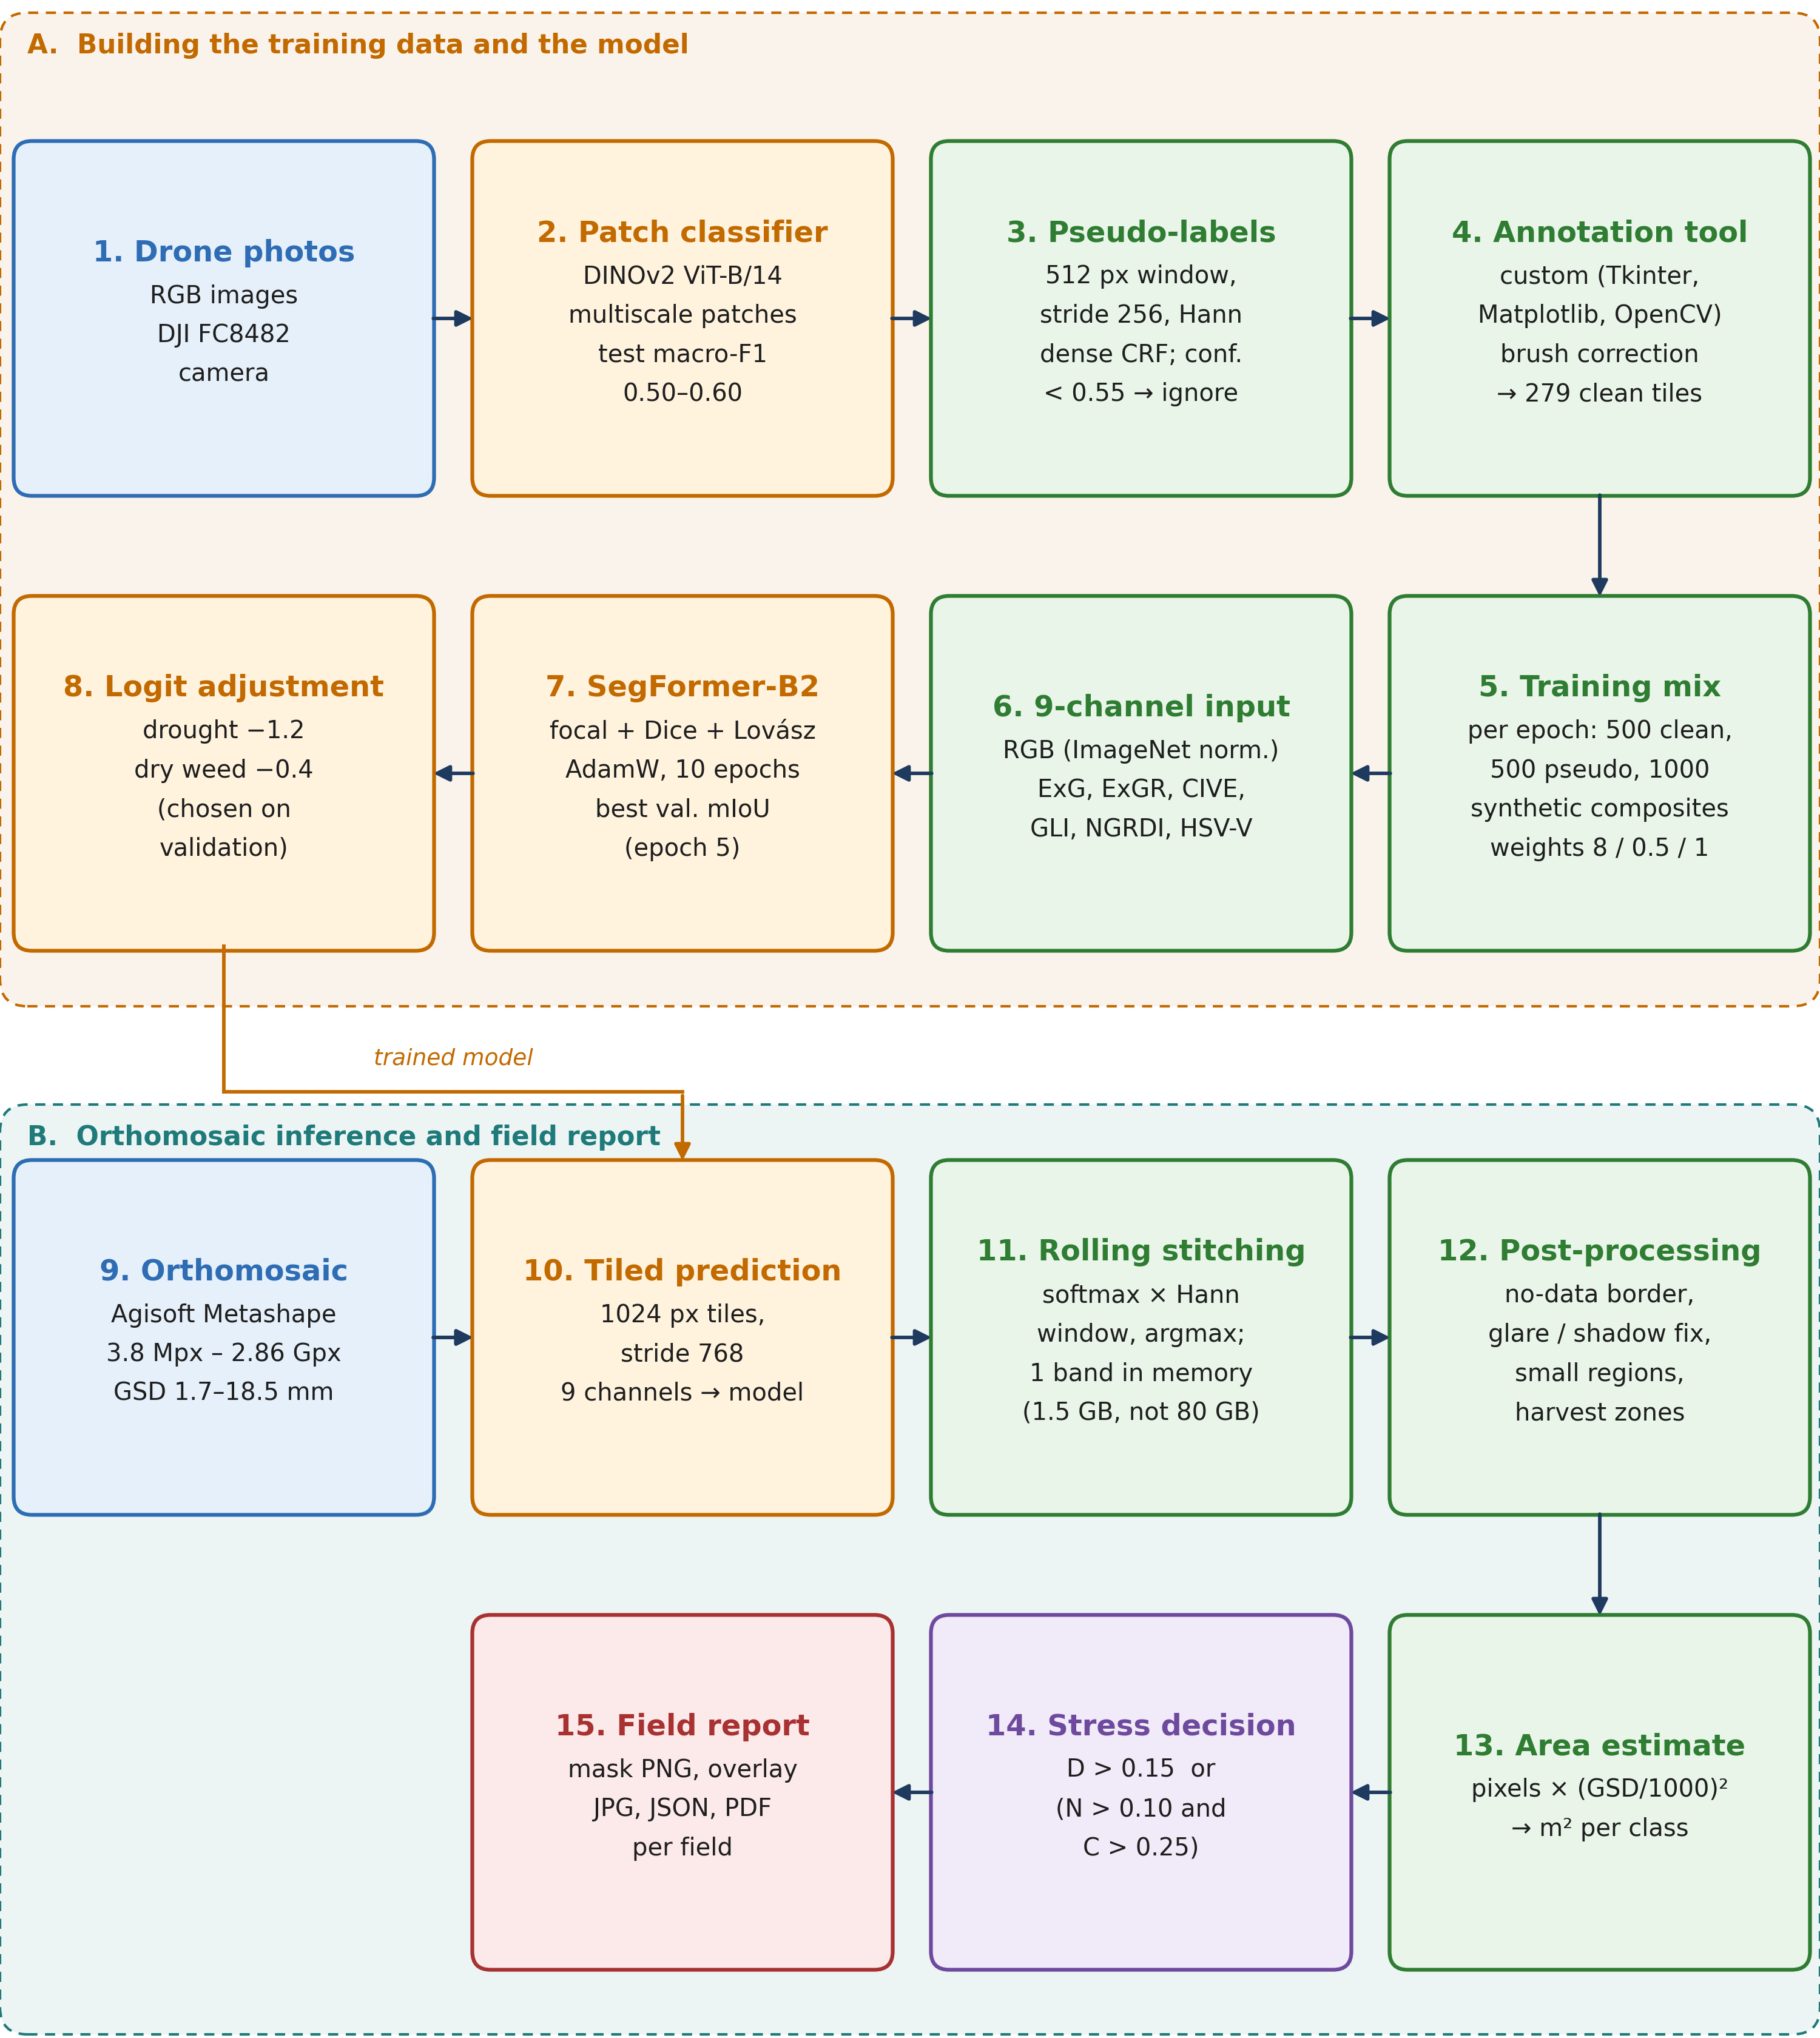
\includegraphics[width=0.93\textwidth]{figures/v2_uav_pipeline.png}
\caption{UAV module from start to end. Steps 1--8 build the labels and the model; steps 9--15 process one field's orthomosaic into a report. Each step is taken from the source code.}
\label{fig:u_pipe}
\end{figure}

\subsection{Data and labels}
Fourteen RGB orthomosaics from drone surveys at the study sites (November 2025 -- January 2026, by the project guide Dr.\ M.\ Naresh Babu and his team) were built with Agisoft Metashape (processed 30 May -- 1 June 2026), from 3.8 million to 2.86 billion pixels. Nine orthomosaics use 98--344 full-resolution photos ($8064\times4536$, DJI FC8482 camera) with ground sampling distance (GSD) 1.68--5.55\,mm; the five Peddakadubur orthomosaics were built from only 8--15 low-resolution frames ($1280\times720$, camera not recorded), hence their coarse GSD of 3.6--18.5\,mm. Seven classes are segmented: background, soil, crop, cotton boll, green weed, dry weed and drought. Labels were built in three steps: (i) a multiscale DINOv2 patch classifier, whose test macro-F1 of only 0.50--0.60 and lack of boundaries motivated segmentation; (ii) its sliding-window predictions (512\,px, stride 256, Hann blending, dense CRF, confidence $\ge 0.55$, else \emph{ignore}) as \textbf{pseudo-labels}; (iii) correction in a \textbf{custom annotation tool} (Python, Tkinter, Matplotlib, OpenCV): the image is shown as a 512\,px grid, the annotator paints classes with a circular brush (radius 2--150\,px, 50-step undo), uncertain pixels stay \emph{ignore} (255), and each tile is saved as image, class mask and overlay. This gave \textbf{279 clean tiles}: 224 for training, 55 for validation (chosen across the range of drought fraction). Training also uses pseudo-labelled crops and \textbf{synthetic composites} (labelled patches pasted onto unlabelled backgrounds: confusing class pairs, small cotton bolls, mixes of 3--7 patches); per epoch 500 clean, 500 pseudo and 1,000 composite samples, with per-sample loss weights 8.0 / 0.5 / 1.0.

\begin{figure}[!htbp]
\centering
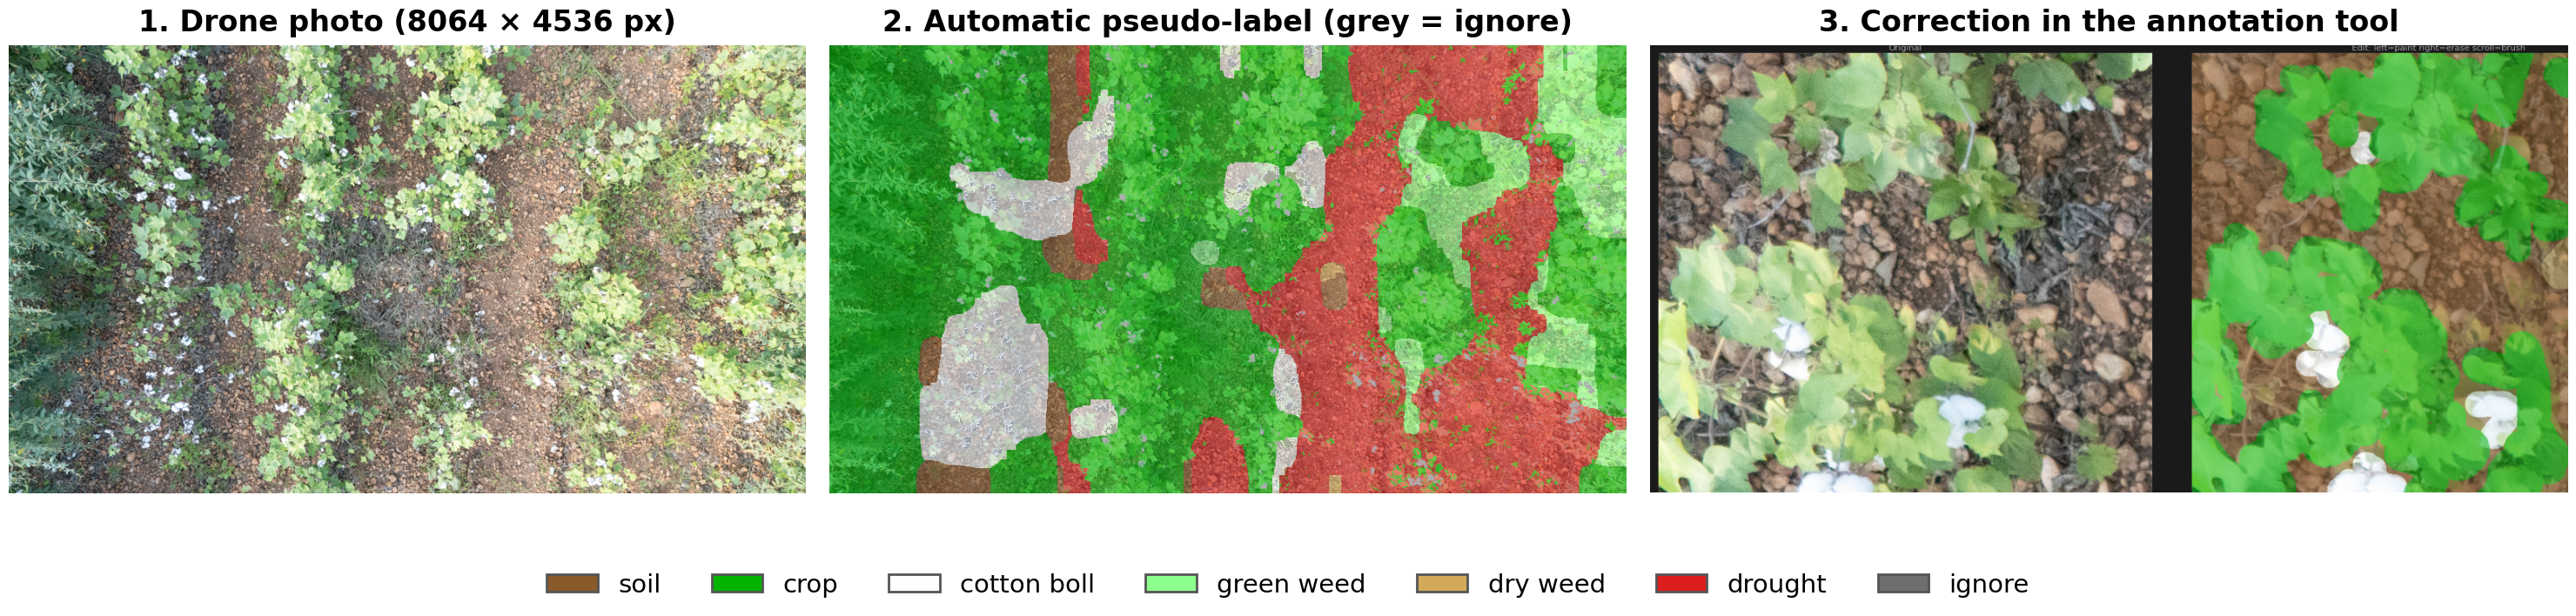
\includegraphics[width=\textwidth]{figures/uav_step_labels.png}
\caption{Building labels on real data. (1) A drone photo of a cotton field. (2) Its automatic pseudo-label from the patch classifier: rough, with many false drought pixels, and uncertain pixels left as \emph{ignore}. (3) Screenshot of the custom annotation tool correcting one tile (left: original, right: editable labels; tile of another photo).}
\label{fig:u_labels}
\end{figure}

\subsection{Model}
Each tile is converted to \textbf{nine channels}: ImageNet-normalised RGB, five vegetation indices computed on RGB in $[0,1]$, and the HSV value $V$ mapped to $[-1,1]$:
\begin{align}
\mathrm{ExG}' &= \frac{2G - R - B}{2}, &
\mathrm{ExGR}' &= \frac{(2G - R - B) - (1.4R - G)}{3}, \\[6pt]
\mathrm{CIVE}' &= -\,\frac{0.441R - 0.811G + 0.385B}{0.811}, &
\mathrm{GLI} &= \frac{2G - R - B}{2G + R + B}, \\[6pt]
\mathrm{NGRDI} &= \frac{G - R}{G + R}, &
V' &= 2V - 1.
\end{align}
Here ExG is the excess-green index, ExGR is ExG minus the excess-red index ($1.4R-G$) and CIVE is the colour index of vegetation extraction; each is rescaled to roughly $[-1,1]$ (primes), and GLI and NGRDI are clipped to $[-1,1]$. The network is \textbf{SegFormer-B2}~\cite{segformer2021} (Fig.~\ref{fig:u_arch}): a Mix-Transformer encoder with four stages (64/128/320/512 channels, depths 3/4/6/3) and an MLP decoder (768) that fuses all stages into 7-class logits at 1/4 resolution, upsampled bilinearly. The ImageNet-pretrained first convolution is widened from 3 to 9 input channels,
\begin{equation}
W_{\text{new}}[:,\,0{:}3] = \tfrac{1}{3}\,W_{\text{old}}, \qquad W_{\text{new}}[:,\,3{:}9] = 0,
\end{equation}
so training starts from the pretrained RGB response.

\begin{figure}[!htbp]
\centering
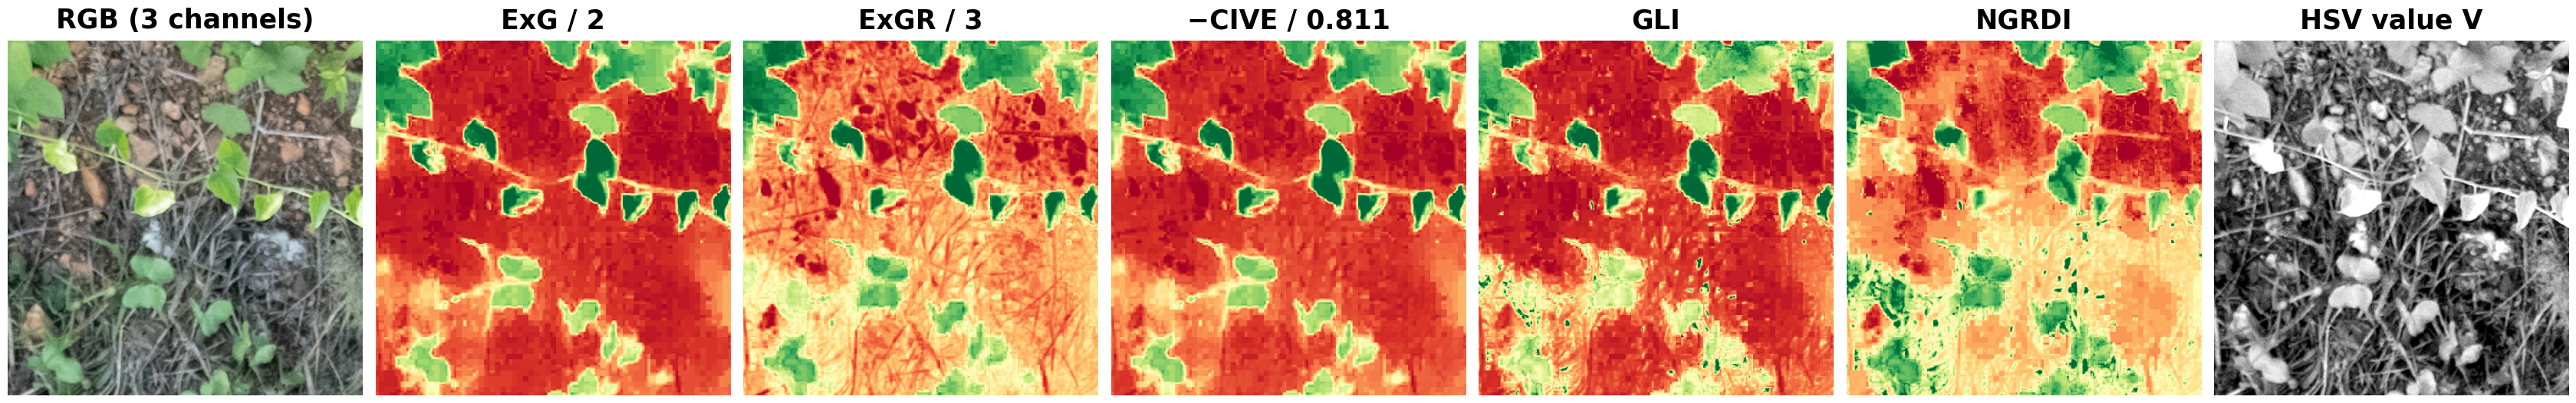
\includegraphics[width=\textwidth]{figures/uav_step_channels.png}
\caption{The nine input channels of one real $512\times512$ tile (green = high vegetation index, red = low). The indices separate green leaves from soil and dry material far more sharply than RGB alone.}
\label{fig:u_channels}
\end{figure}

\begin{figure}[!htbp]
\centering
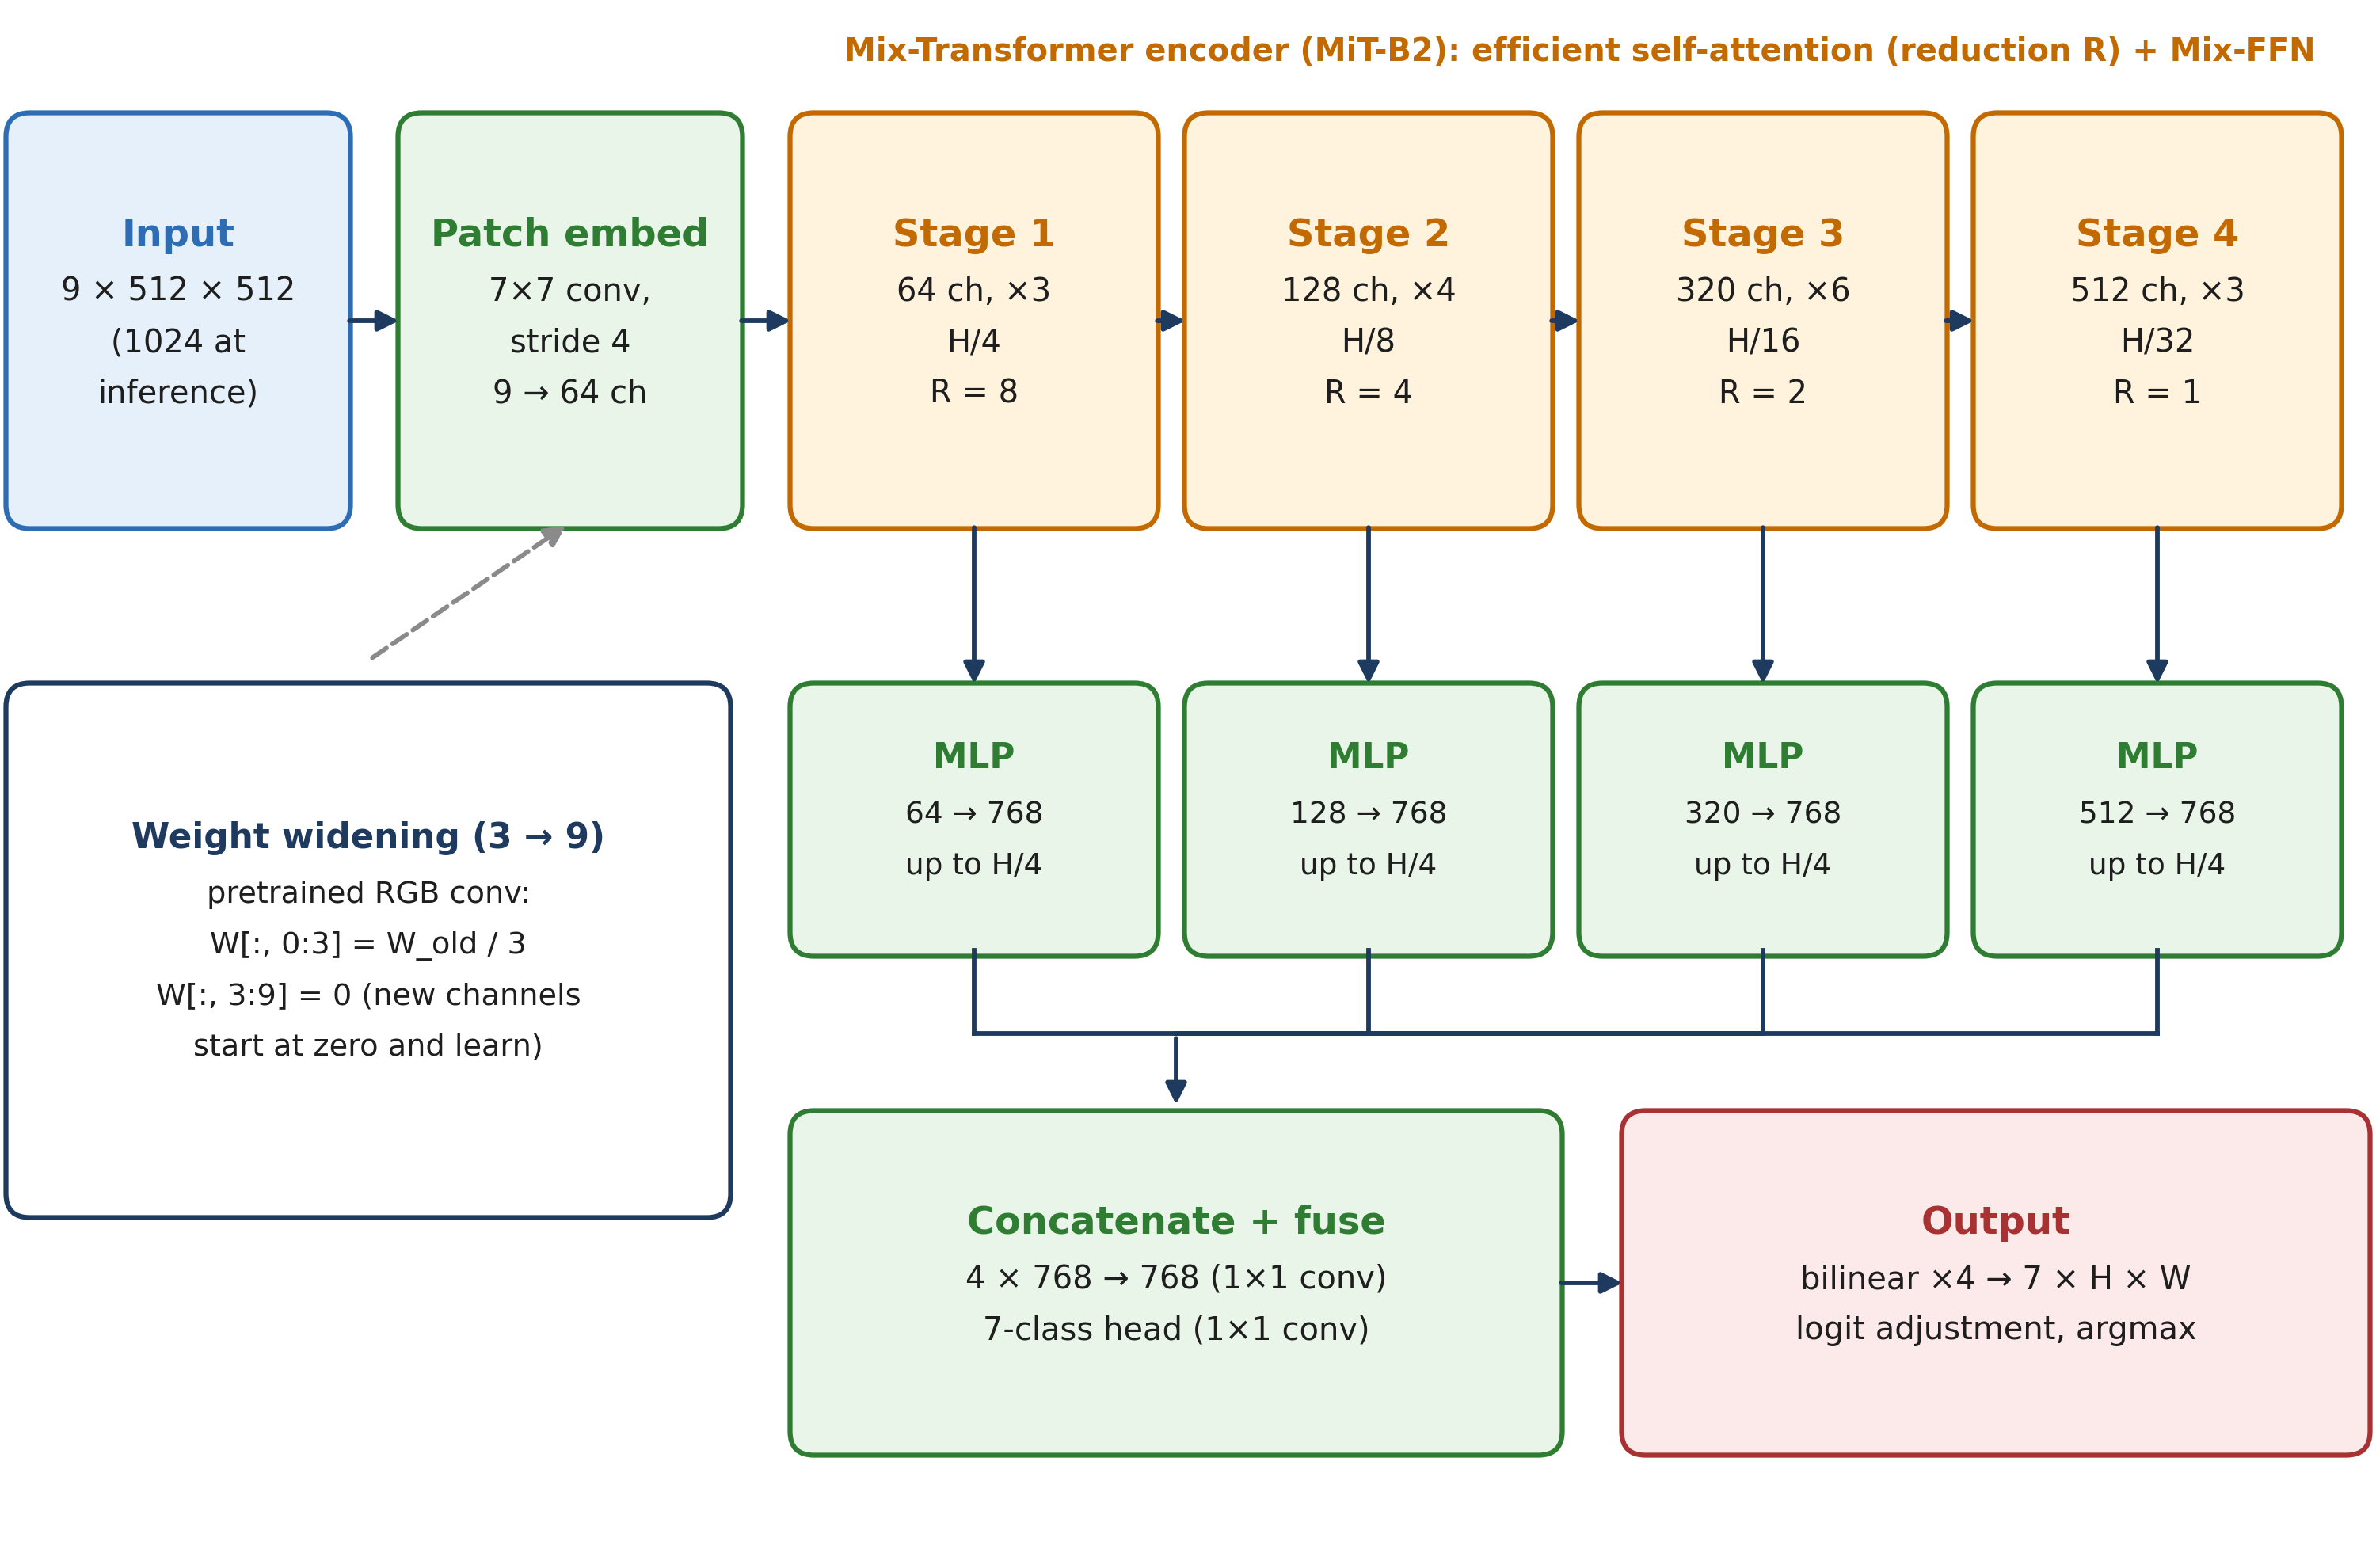
\includegraphics[width=0.95\textwidth]{figures/v2_uav_model.png}
\caption{UAV segmentation model: nine-channel SegFormer-B2. Stage settings (channels, depth, resolution, attention reduction R) as in the source code and the MiT-B2 defaults it loads.}
\label{fig:u_arch}
\end{figure}

\subsection{Training}
The loss combines focal, Dice and Lov\'asz-Softmax terms (ignore pixels excluded):
\begin{equation}
\mathcal{L} = 1.0\,\mathcal{L}_{\text{focal}}(\gamma{=}2) + 2.5\,\mathcal{L}_{\text{Dice}} + 1.0\,\mathcal{L}_{\text{Lov\'asz}}, \qquad
\mathcal{L}_{\text{focal}} = -\alpha_{y}(1-p_y)^{\gamma}\log p_y,
\end{equation}
with inverse-frequency class weights $\alpha_c = N/(C\,N_c)$ clipped to $[0.1, 50]$, drought set to 10 and cotton boll to 8 (training pixels: soil 45\,\%, green weed 18\,\%, crop 14\,\%, dry weed 12\,\%, drought 10\,\%, cotton 0.3\,\%). Optimiser AdamW (learning rate $2\!\times\!10^{-6}$, weight decay 0.01, cosine decay, gradient clipping 1.0), batch 16, 10 epochs, augmentation by flips, 90$^\circ$ rotations and HSV jitter. The checkpoint with the best validation mIoU (epoch 5) is kept. The very low learning rate and 60.9\,\% mIoU after the first epoch indicate fine-tuning of an earlier checkpoint whose identity was not recorded.

\textbf{Logit adjustment.} The raw model over-predicts drought (recall 95\,\%, precision 54\,\%). At inference 1.2 is subtracted from the drought logit and 0.4 from the dry-weed logit; the drought value was chosen from a sweep (0--2.0) on the validation tiles, so the adjusted scores are optimistic.

\subsection{Orthomosaic inference, area and decision}
Orthomosaics are processed in $1024\times1024$ tiles with stride 768. Overlapping softmax outputs are blended with a 2-D Hann window $w$, $A_c(x) = \sum_i w_i(x)\,p_{i,c}(x)$, and the class is $\arg\max_c A_c(x)$. A \textbf{rolling accumulator} keeps only one tile-height band in memory ($O(C\,T\,W)$ instead of $O(C\,H\,W)$): for the largest orthomosaic this is 1.47\,GB instead of 80\,GB. Post-processing removes no-data borders, relabels glare and shadow pixels by their 9$\times$9 majority, removes small components (drought $<$ 200\,px) and tags harvest zones (cotton-boll density $>$ 5\,\% in 256\,px windows); images above $10^8$ pixels use a block-wise, disk-backed version (equivalence tests: 21/21, 18/18, 24/24 passed, zero mask differences on the same GPU). Class area is $N_c\,(\mathrm{GSD}/1000)^2$ m$^2$. With $D$ = drought share of the agricultural area (crop, cotton, dry weed, drought), $N$ = the same outside harvest zones, and $C$ = share of drought pixels in the largest drought region, a field gets a \textbf{visual stress flag} if $D > 0.15$ or ($N > 0.10$ and $C > 0.25$). The accompanying score $\min\!\big(1, 0.5D/0.15 + 0.3N/0.10 + 0.2\,[C>0.25]\big)$ is a heuristic, not a probability.

\begin{figure}[!htbp]
\centering
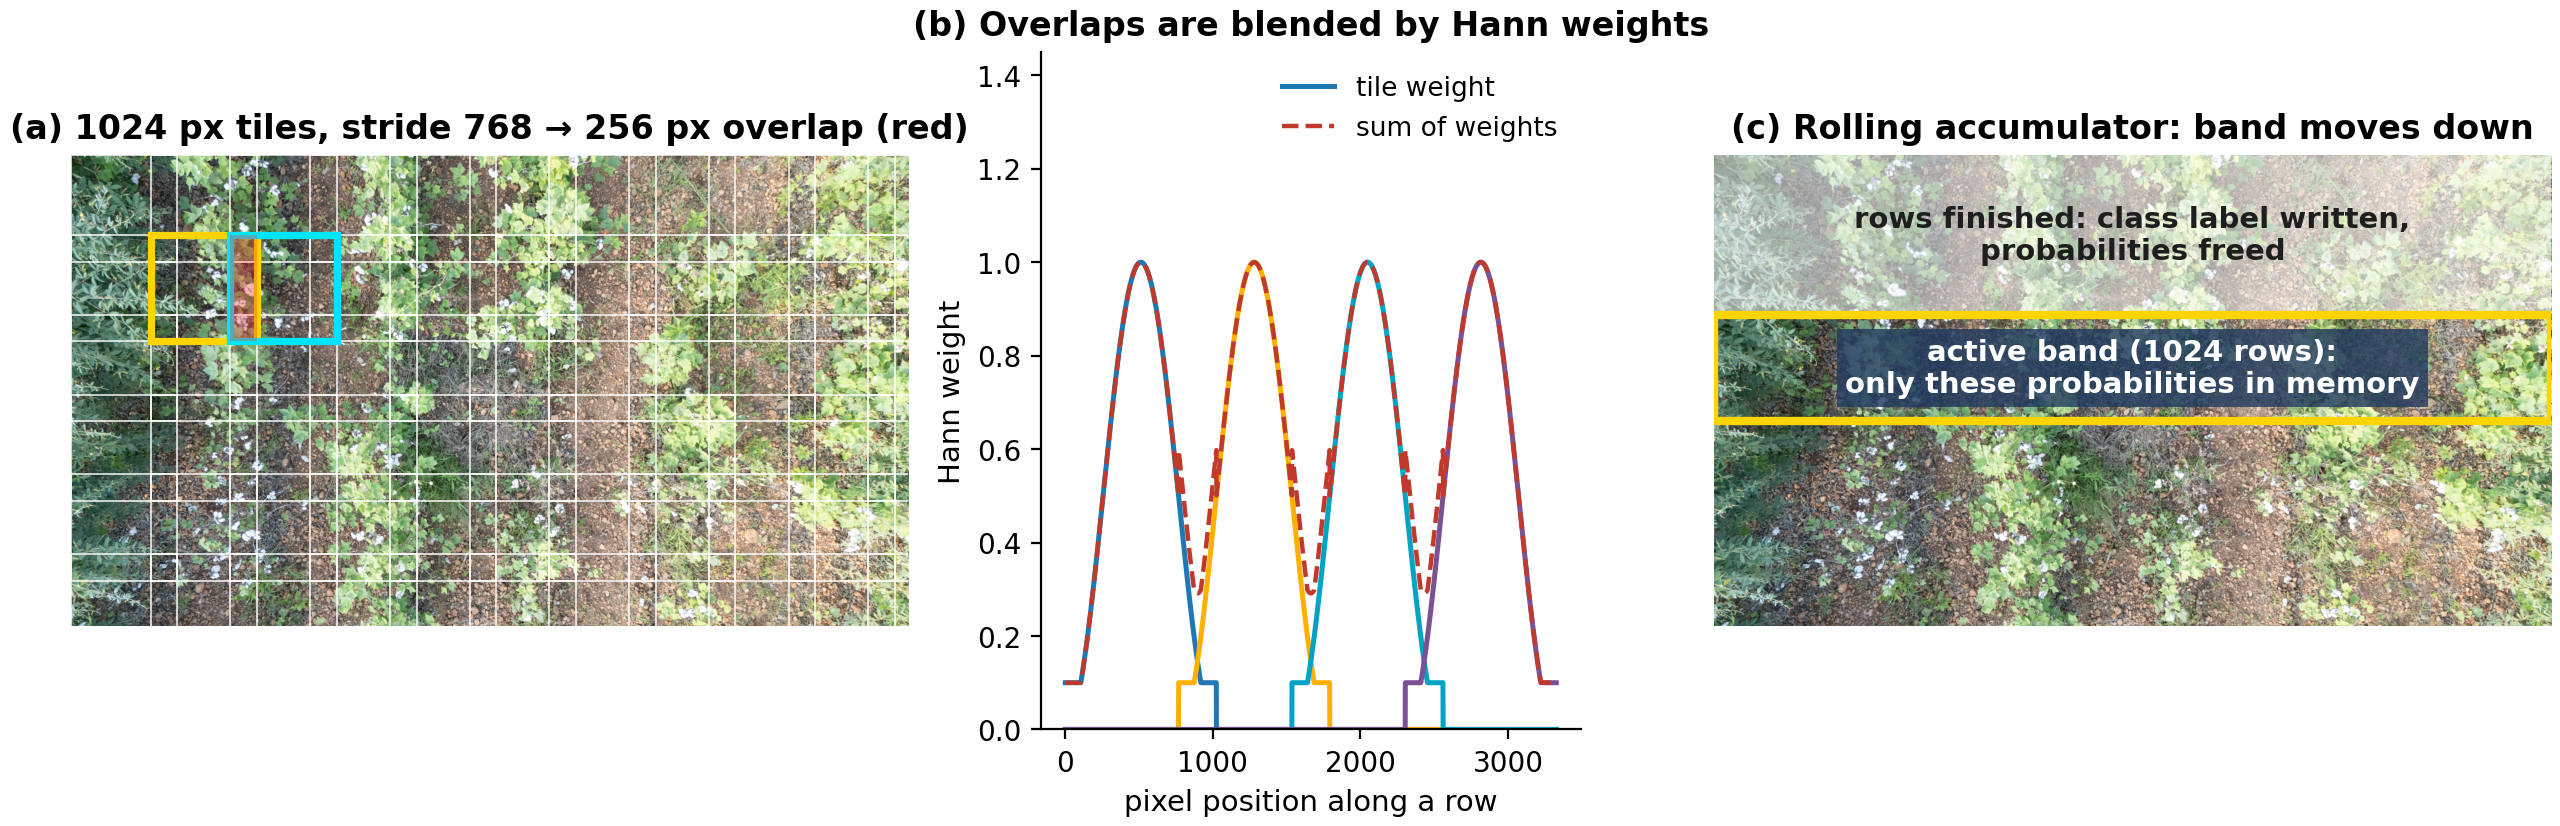
\includegraphics[width=\textwidth]{figures/uav_step_stitching.png}
\caption{How prediction stitching works (shown on one drone photo; an orthomosaic is processed the same way). (a) The image is cut into overlapping $1024$\,px tiles. (b) Each tile's class probabilities are weighted by a Hann window (high in the centre, low at the edges, clamped at 0.1), so tile borders do not create seams. (c) Only one 1024-row band of probabilities is kept in memory; rows above it are final.}
\label{fig:u_stitch}
\end{figure}

\subsection{Results}
\begin{table}[H]
\centering
\caption{UAV segmentation on the 55 validation tiles (mIoU = mean IoU of the 6 foreground classes). Not an independent test.}
\label{tab:u_val}
\footnotesize
\begin{tabular}{|l|c|l|c|c|}
\hline
\textbf{Model version} & \textbf{mIoU} & \textbf{V11, metric} & \textbf{raw} & \textbf{adjusted} \\
\hline
V8, SegFormer-B2 & 61.18 & mIoU & 61.46 & \textbf{65.11} \\ \hline
V9 / V9.1, SegFormer-B3 & 44.25 / 45.89 & Pixel accuracy & 78.81 & \textbf{82.68} \\ \hline
V10, DeepLabV3+ & 44.79 & Macro F1 & 75.75 & 78.51 \\ \hline
\textbf{V11, SegFormer-B2} & \textbf{61.46} & Drought precision / recall & 54.4 / 95.5 & 76.4 / 82.1 \\ \hline
V12, SegFormer-B2 & 61.39 & Drought F1 / IoU & 69.3 / 53.0 & 79.2 / 65.5 \\
\hline
\end{tabular}
\end{table}
SegFormer-B2 clearly beats B3 and DeepLabV3+ in these runs, although the runs differ in settings and are not a controlled comparison; V11 is only 0.3 points above V8. Logit adjustment trades drought recall for precision and raises drought IoU by 12.5 points. A provenance audit found that 22 of the 55 validation tiles share a source photograph with training tiles; on the 33 source-disjoint tiles the adjusted mIoU is 69.3\,\% (overlapping tiles 45.1\,\%), so overlap does not inflate the headline number, but no independent test exists yet.

Per-class IoU after adjustment: soil 74, crop 73, cotton boll 53, green weed 71, dry weed 54, drought 65\,\%. The confusion matrix (Fig.~\ref{fig:u_conf}) shows that the remaining drought errors go mostly to soil (8.8\,\%) and green weed (6.2\,\%), and that dry weed is the hardest class (15\,\% predicted as soil, 11\,\% as green weed); drought and dry weed are rarely confused with each other (1.4--1.8\,\%).

\begin{figure}[!htbp]
\centering
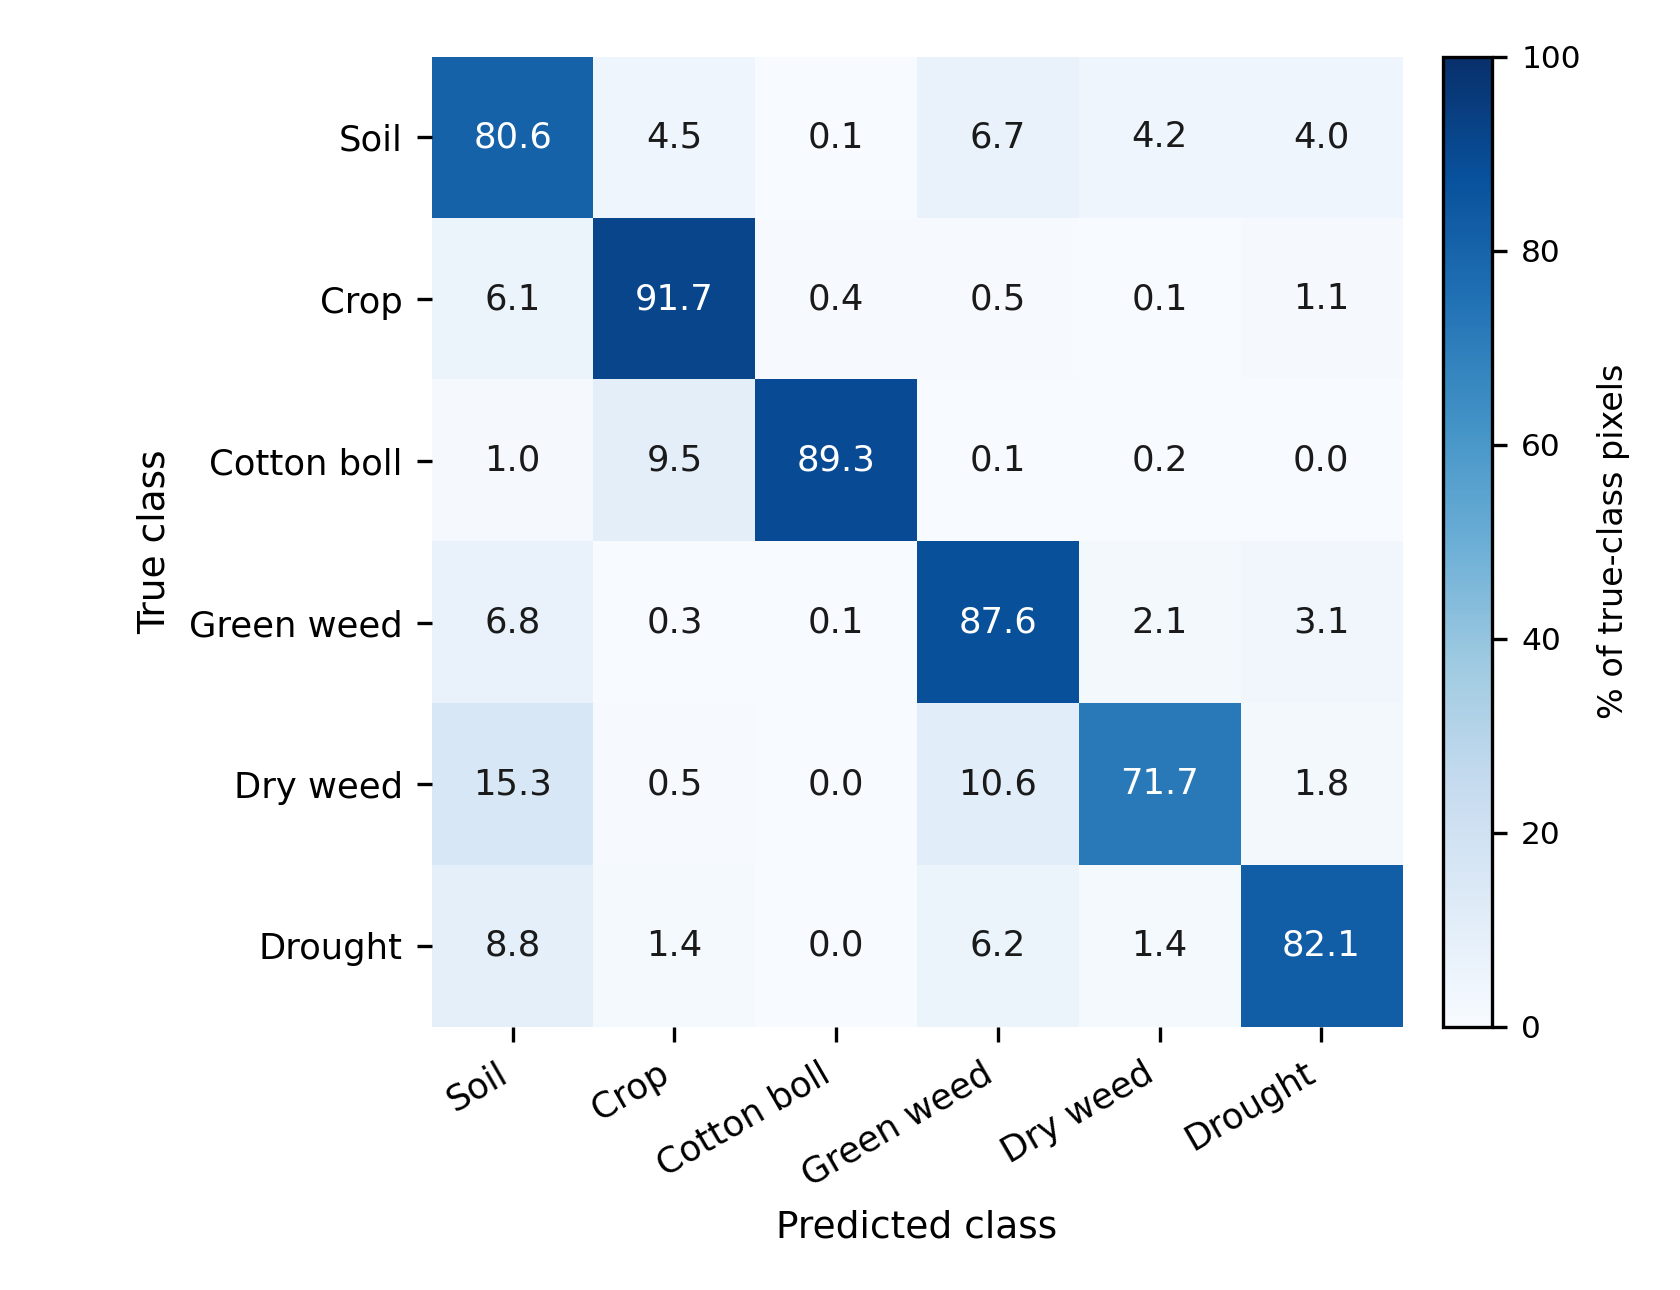
\includegraphics[width=0.7\textwidth]{figures/uav_confusion.png}
\caption{UAV validation confusion matrix after logit adjustment (row-normalised, 55 validation tiles).}
\label{fig:u_conf}
\end{figure}

\begin{table}[!htbp]
\centering
\caption{Field results on the 14 orthomosaics (V11, adjusted). Drought = share of the agricultural area. Areas are estimates: no field has a verified physical scale.}
\label{tab:u_fields}
\scriptsize
\setlength{\tabcolsep}{3.5pt}
\begin{tabular}{|l|r|r|r|r|c|l|r|r|r|r|c|}
\hline
\textbf{Field} & \textbf{GSD} & \textbf{Area} & \textbf{Drought} & \textbf{Score} & \textbf{Flag} & \textbf{Field} & \textbf{GSD} & \textbf{Area} & \textbf{Drought} & \textbf{Score} & \textbf{Flag} \\ \hline
 & mm & m$^2$ & \% & \% & & & mm & m$^2$ & \% & \% & \\
\hline
Lepakshi & 2.08 & 2,976 & 71.53 & 100 & \textbf{yes} & Pulliah & 2.69 & 2,897 & 0.04 & 20 & no \\ \hline
Sira & 2.14 & 4,341 & 54.26 & 100 & \textbf{yes} & Balaji Villas & 1.84 & 8,044 & 0.06 & 20 & no \\ \hline
Somandepalle & 2.35 & 3,936 & 25.45 & 100 & \textbf{yes} & Shilpa & 1.94 & 6,395 & 0.00 & 20 & no \\ \hline
KNL Puddur & 1.73 & 3,866 & 0.15 & 1 & no & KNL DDP & 5.55 & 19,812 & 0.00 & 20 & no \\ \hline
KNL Maize Tower & 1.68 & 2,241 & 0.07 & 21 & no & Peddakadubur F3 & 4.34 & 61 & 0.89 & 26 & no \\ \hline
Peddakadubur F1, F4 & 3.6, 9.2 & 42, 276 & 0, 0 & 0 & no & Peddakadubur F6, F7 & 18.5, 10.4 & 660, 431 & 0, 0 & 0 & no \\
\hline
\end{tabular}
\end{table}

\begin{figure}[!htbp]
\centering
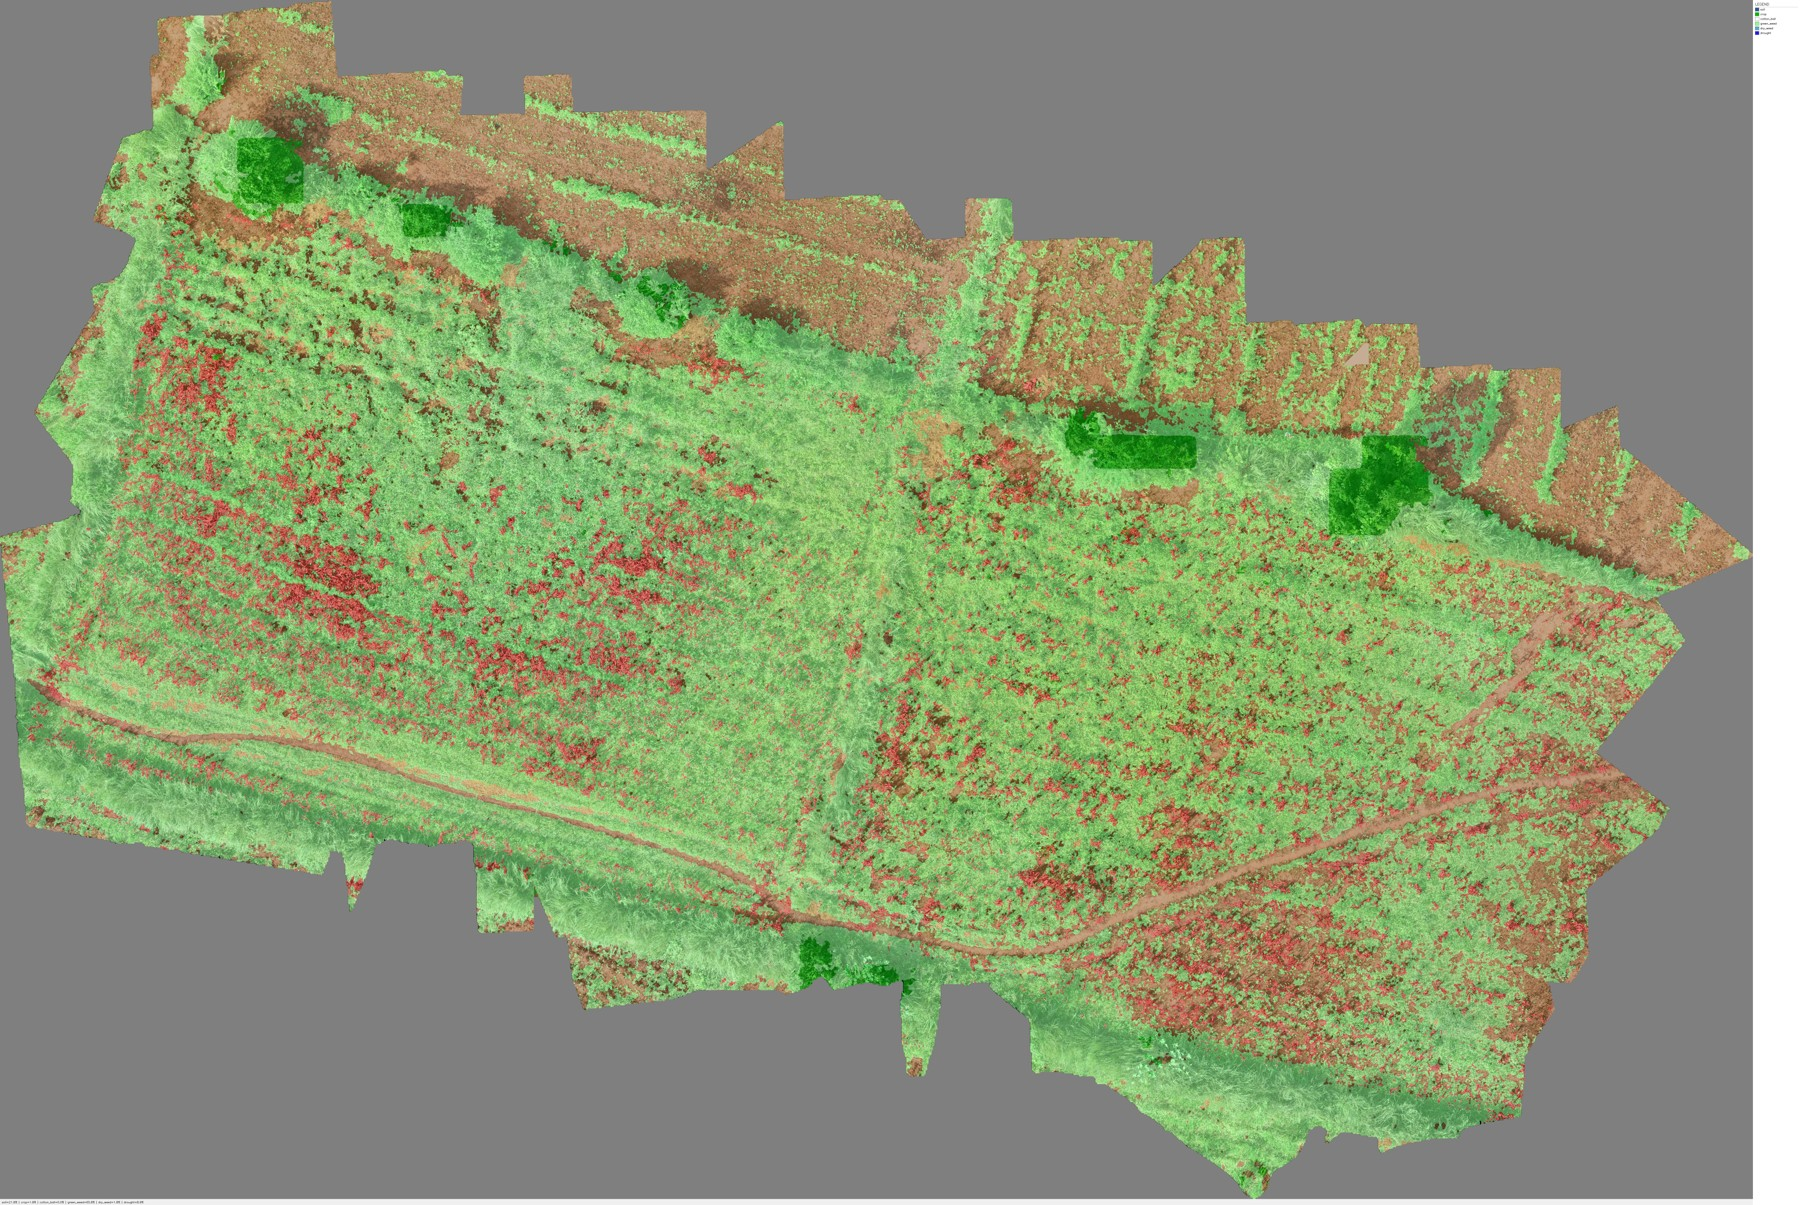
\includegraphics[width=0.78\textwidth]{figures/uav_lepakshi_overlay.jpg}
\caption{Lepakshi orthomosaic with the V11 prediction overlaid (red = drought, light green = green weed, brown = soil, dark green = crop). 71.5\,\% of the agricultural area is predicted as drought, so the field is flagged.}
\label{fig:u_overlay}
\end{figure}

\begin{figure}[!htbp]
\centering
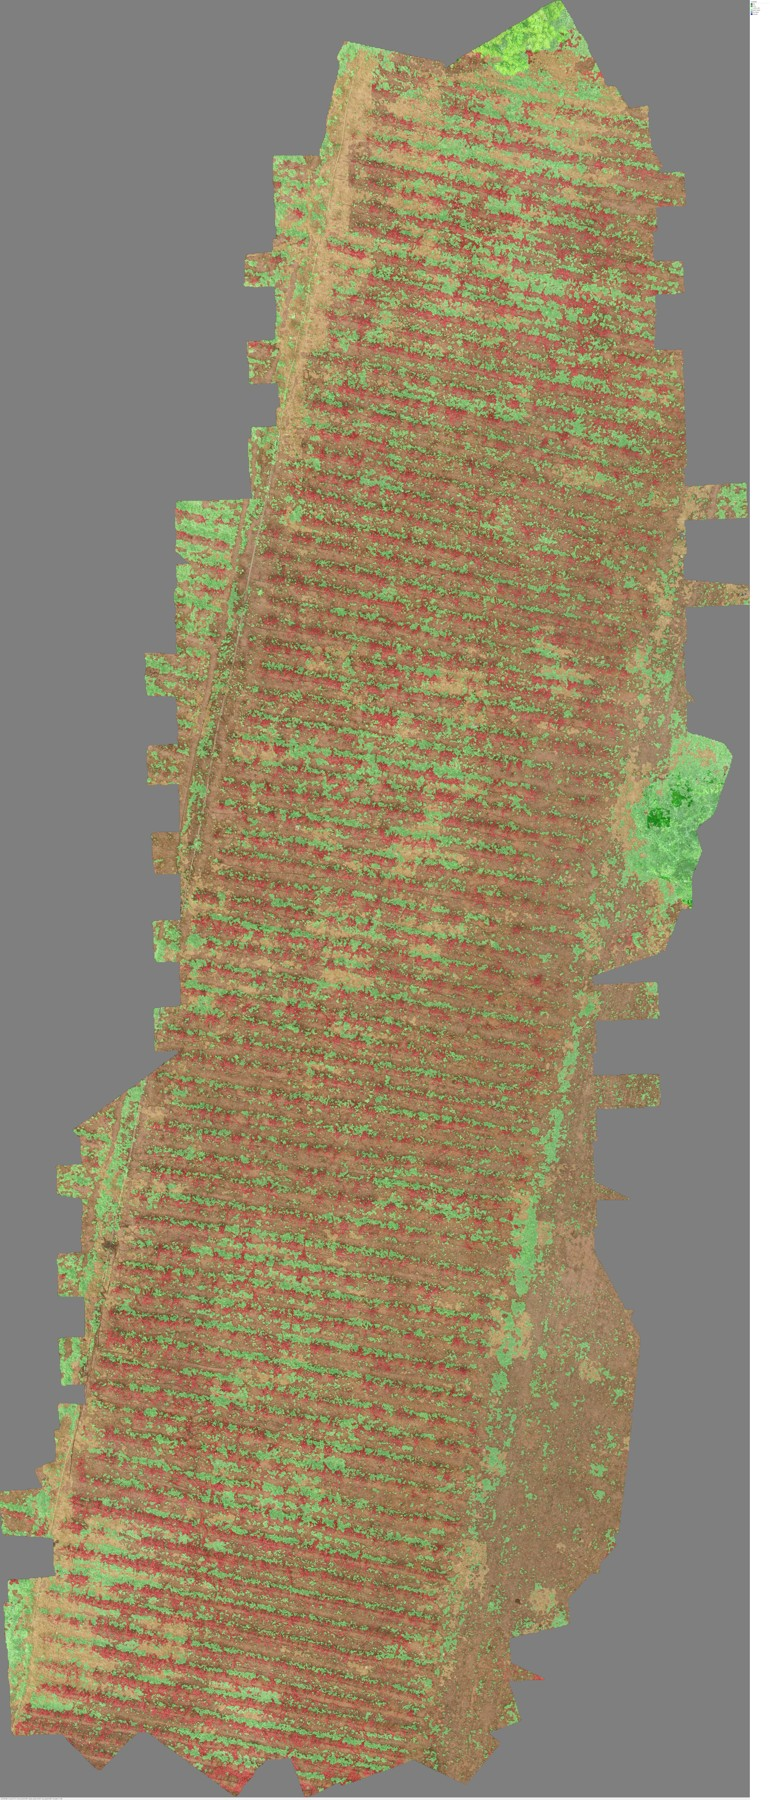
\includegraphics[height=8.2cm]{figures/uav_sira_overlay.jpg}\hspace{1.2cm}
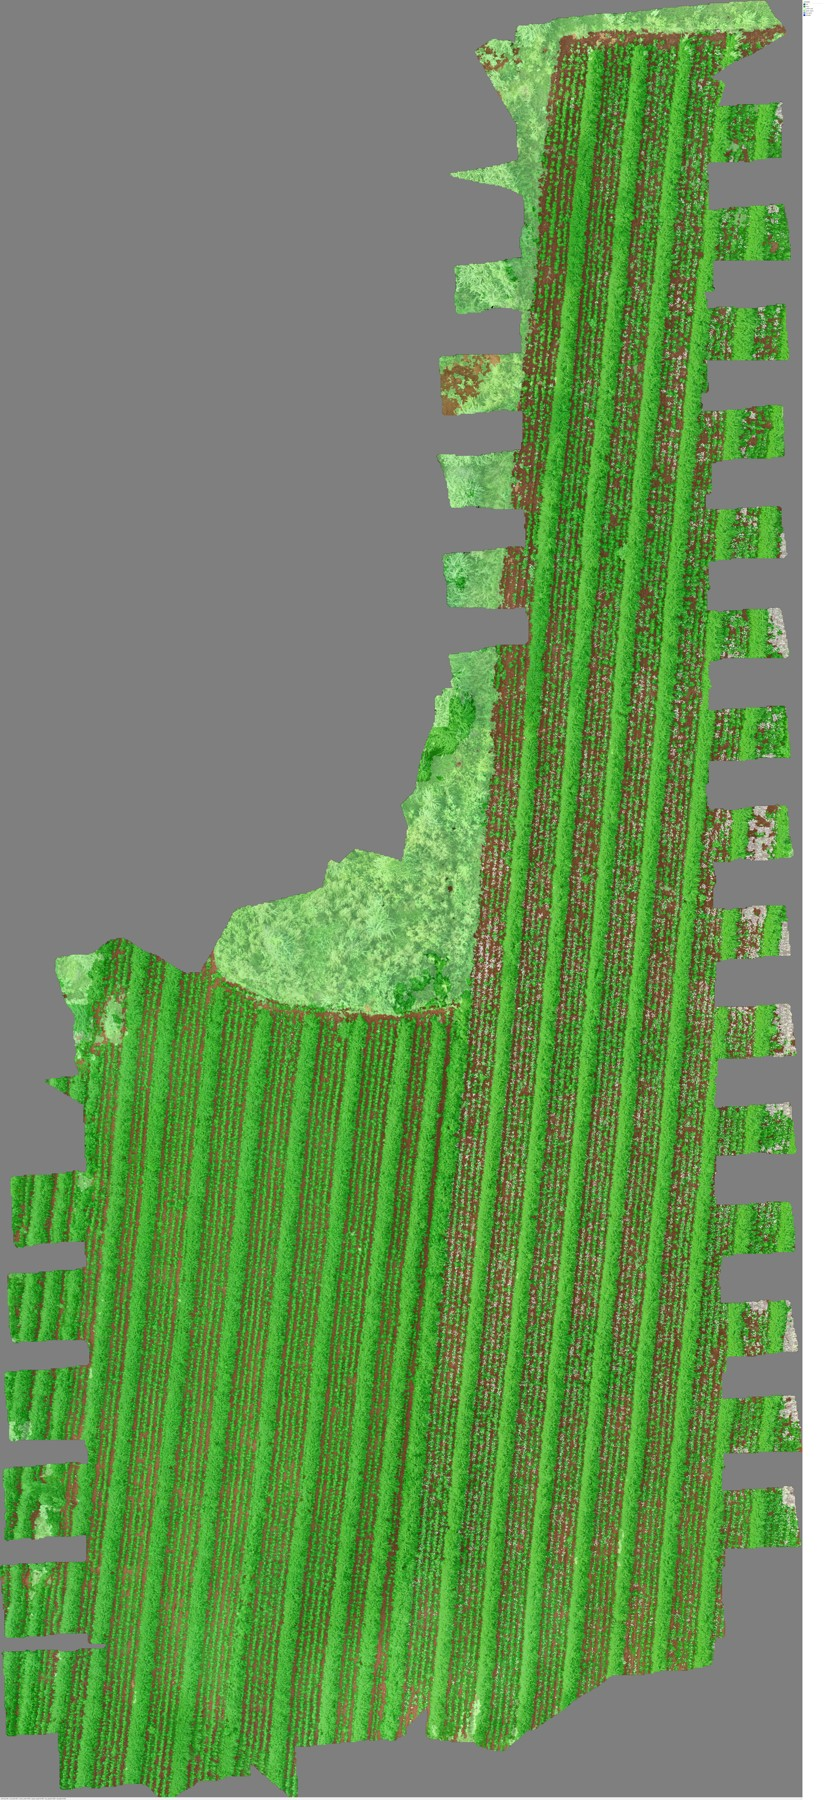
\includegraphics[height=8.2cm]{figures/uav_knlddp_overlay.jpg}
\caption{Flagged vs not flagged. Left: Sira (54.3\,\% of the agricultural area predicted as drought, red). Right: KNL DDP cotton field (0.0004\,\% drought; crop rows dark green, soil brown, field margins green weed).}
\label{fig:u_pair}
\end{figure}

All 14 orthomosaics were processed (56 output files: mask, overlay, JSON and PDF per field). The three flagged fields (Lepakshi, Sira, Somandepalle) are the southern fields that the survey team also judged drought-affected (Table~\ref{tab:s_uav_short}); none of the Kurnool fields is flagged. On the largest orthomosaic (2.86 billion pixels) inference took 45 minutes on an NVIDIA L4 GPU. An earlier run of the KNL DDP orthomosaic took 98 minutes on an A100 against 25 minutes for the optimised pipeline on a T4; the hardware differs, so this is not a controlled speed comparison.

\begin{table}[H]
\centering
\caption{Survey-team field verdicts vs the UAV flag and the Sentinel-2 verdict at the flight date (satellite comparison from Module 2).}
\label{tab:s_uav_short}
\scriptsize
\begin{tabular}{|l|l|l|l|}
\hline
\textbf{Field} & \textbf{Survey verdict} & \textbf{UAV module flag} & \textbf{Satellite (SVI)} \\
\hline
Lepakshi, Somandepalle (maize) & drought & flagged & not stressed \\ \hline
Sira (cotton + maize) & drought / healthy & flagged & not stressed \\ \hline
Balaji Villas, Pullaiah (cotton) & healthy & not flagged & stressed \\ \hline
Dinnedevarapadu, Shilpa, Puddur & healthy & not flagged & not stressed \\ \hline
Peddakadubur (cotton) & mixed & not flagged & not stressed \\
\hline
\end{tabular}
\end{table}
The drone sees what the 10\,m satellite pixel cannot: patchy drought inside a field that is green on average, and post-harvest fields that the satellite reads as stressed.

% ============================================================================
\section{Conclusion, Limitations and Future Work}
We built and evaluated a three-module drought framework with honest baselines. In \textbf{kharif}, the hybrid weather model forecasts the SPEI-30 class with \mf{} 0.819 / 0.651 at 7 / 15 days, rainfed crops respond about 10 days later, and the weather-to-satellite chain confirmed all 9 severe declared droughts of 2023--2026, five before the order. In \textbf{rabi}, a soil-moisture deficit-duration indicator relates to independent crop yields and warns of loss seasons by mid-December (AUC 0.80), confirmed by MODIS greenness on 13 independent seasons (AUC 0.83); a field model warns of early drying up to 30 days ahead, and its warnings are about twice as reliable under dry soil. The \textbf{UAV} module segments multi-billion-pixel orthomosaics into 7 classes (validation mIoU 65.1\,\%) and flags the three fields the survey team judged drought-hit.

\textbf{Limitations.} No module is validated against field-level drought measurements; government orders and district yields are indirect. Nothing is skilful 30 days ahead in kharif. Rabi yield validation covers 2 districts and 23 seasons, and the field early-drying test had only one dry season. UAV metrics come from validation tiles (22 of 55 share source photographs, adjustment tuned on them); RGB shows visual stress, not its cause; GSD and acquisition dates of the orthomosaics are not independently verified; the stress score is not a probability.

\textbf{Future work.} (i) Run the full kharif/rabi $\rightarrow$ UAV loop in rabi 2026-27 with the frozen rules; (ii) complete the 127-tile independent UAV test set with human labels and field confirmation; (iii) a trend-robust greenness reference for rabi; (iv) multispectral or thermal UAV imagery.

\textbf{Code:} github.com/ARYAN3012-G/weather\_time\_series $\cdot$ github.com/ARYAN3012-G/Sentinel2-Drought-Confirmation $\cdot$ github.com/ARYAN3012-G/Rabi-Drought-Monitoring-

% ============================================================================
\section*{References}
\addcontentsline{toc}{section}{References}
\begingroup
\footnotesize
\setlength{\parskip}{0pt}
\renewcommand{\section}[2]{}
\begin{thebibliography}{30}
\setlength{\itemsep}{0pt}
\setlength{\parsep}{0pt}
\bibitem{manual2016} Government of India, \textit{Manual for Drought Management}, Ministry of Agriculture and Farmers Welfare, 2016 (updated 2020).
\bibitem{bhardwaj2021} K.~Bhardwaj and V.~Mishra, ``Drought detection and declaration in India,'' \textit{Water Security}, vol.~14, p.~100104, 2021.
\bibitem{vicente2010} S.~M.~Vicente-Serrano, S.~Beguer\'{i}a, and J.~I.~L\'{o}pez-Moreno, ``A multiscalar drought index sensitive to global warming: the Standardized Precipitation Evapotranspiration Index,'' \textit{J.\ Climate}, vol.~23, no.~7, pp.~1696--1718, 2010.
\bibitem{dikshit2021} A.~Dikshit, B.~Pradhan, and A.~Huete, ``An improved SPEI drought forecasting approach using the long short-term memory neural network,'' \textit{J.\ Environ.\ Manage.}, vol.~283, p.~111979, 2021.
\bibitem{marusov2024} A.~Marusov, V.~Grabar, Y.~Maximov \textit{et al.}, ``Long-term drought prediction using deep neural networks based on geospatial weather data,'' \textit{Environ.\ Model.\ Softw.}, vol.~179, 2024.
\bibitem{allen1998} R.~G.~Allen, L.~S.~Pereira, D.~Raes, and M.~Smith, \textit{Crop Evapotranspiration}, FAO Irrigation and Drainage Paper 56, Rome, 1998.
\bibitem{agera5} H.~Boogaard \textit{et al.}, ``Agrometeorological indicators from 1979 to present derived from reanalysis (AgERA5),'' Copernicus Climate Change Service Climate Data Store.
\bibitem{chen2016} T.~Chen and C.~Guestrin, ``XGBoost: a scalable tree boosting system,'' in \textit{Proc.\ ACM SIGKDD}, pp.~785--794, 2016.
\bibitem{breiman2001} L.~Breiman, ``Random forests,'' \textit{Machine Learning}, vol.~45, no.~1, pp.~5--32, 2001.
\bibitem{kogan1995} F.~N.~Kogan, ``Application of vegetation index and brightness temperature for drought detection,'' \textit{Adv.\ Space Res.}, vol.~15, no.~11, pp.~91--100, 1995.
\bibitem{peters2002} A.~J.~Peters \textit{et al.}, ``Drought monitoring with NDVI-based Standardized Vegetation Index,'' \textit{Photogramm.\ Eng.\ Remote Sens.}, vol.~68, no.~1, pp.~71--75, 2002.
\bibitem{prodhan2021} F.~A.~Prodhan, J.~Zhang, F.~Yao \textit{et al.}, ``Deep learning for monitoring agricultural drought in South Asia using remote sensing data,'' \textit{Remote Sens.}, vol.~13, no.~9, p.~1715, 2021.
\bibitem{sharma2025} S.~S.~Sharma, J.~Mukherjee, and F.~Dell'Acqua, ``Leveraging Sentinel-2 data and machine learning for drought detection in India,'' \textit{Remote Sens.}, vol.~17, no.~18, p.~3159, 2025.
\bibitem{danodia2021} A.~Danodia, A.~Kushwaha, and N.~R.~Patel, ``Remote sensing-derived combined index for agricultural drought assessment of rabi pulse crops in Bundelkhand region, India,'' \textit{Environ.\ Dev.\ Sustain.}, vol.~23, no.~10, pp.~15432--15449, 2021.
\bibitem{nikam2020} B.~R.~Nikam \textit{et al.}, ``Assessment of early season agricultural drought using remote sensing,'' \textit{ISPRS Arch.}, vol.~XLIII-B3-2020, pp.~1691--1695, 2020.
\bibitem{descals2025} A.~Descals, K.~Torres, A.~Verger, and J.~Pe\~{n}uelas, ``Evaluating Sentinel-2 for monitoring drought-induced crop failure in winter cereals,'' \textit{Remote Sens.}, vol.~17, no.~2, p.~340, 2025.
\bibitem{kulkarni2020} S.~S.~Kulkarni, B.~D.~Wardlow, Y.~A.~Bayissa, T.~Tadesse, M.~D.~Svoboda, and S.~S.~Gedam, ``Developing a remote sensing-based combined drought indicator approach for agricultural drought monitoring over Marathwada, India,'' \textit{Remote Sens.}, vol.~12, no.~13, p.~2091, 2020.
\bibitem{gorelick2017} N.~Gorelick \textit{et al.}, ``Google Earth Engine: planetary-scale geospatial analysis for everyone,'' \textit{Remote Sens.\ Environ.}, vol.~202, pp.~18--27, 2017.
\bibitem{drusch2012} M.~Drusch \textit{et al.}, ``Sentinel-2: ESA's optical high-resolution mission for GMES operational services,'' \textit{Remote Sens.\ Environ.}, vol.~120, pp.~25--36, 2012.
\bibitem{achanta2017} R.~Achanta and S.~S\"{u}sstrunk, ``Superpixels and polygons using simple non-iterative clustering,'' in \textit{Proc.\ CVPR}, 2017.
\bibitem{segformer2021} E.~Xie, W.~Wang, Z.~Yu, A.~Anandkumar, J.~M.~Alvarez, and P.~Luo, ``SegFormer: simple and efficient design for semantic segmentation with Transformers,'' in \textit{Proc.\ NeurIPS}, 2021.
\bibitem{niu2024} H.~Niu, J.~Landivar, and N.~Duffield, ``Classification of cotton water stress using convolutional neural networks and UAV-based RGB imagery,'' \textit{Adv.\ Modern Agric.}, vol.~5, no.~1, 2024.
\bibitem{shahi2023} T.~B.~Shahi, S.~Dahal, C.~Sitaula, A.~Neupane, and W.~Guo, ``Deep learning-based weed detection using UAV images: a comparative study,'' \textit{Drones}, vol.~7, no.~10, p.~624, 2023.
\end{thebibliography}
\endgroup

\vspace{8pt}
\noindent\rule{0.38\textwidth}{0.4pt}\hfill\rule{0.28\textwidth}{0.4pt}\\[2pt]
\noindent\textbf{Guide's Signature}\hfill\textbf{Date}
\end{document}
